% !TEX TS-program = pdflatex
% !TEX encoding = UTF-8 Unicode

% for proofreading the text
%\documentclass[10pt,twocolumn,article,draft]{memoir}
\documentclass[10pt,twocolumn,article]{memoir}

%% closer to real thesis format
%\documentclass[12pt,letterpaper]{memoir}
%\OnehalfSpacing

% 1in margins everywhere. I do this for proofreading too, so that I can see exactly how the figures will look on their pages in the final document
\settypeblocksize{9in}{6.5in}{*}
\setlrmargins{1.0in}{*}{*}
\setulmargins{1.0in}{*}{*}
\checkandfixthelayout

\usepackage{thesis}
\usepackage{tikz} % drawing figures right here in this file!

% number equations, tables, and figures by chapter
\numberwithin{equation}{chapter}
\numberwithin{figure}{chapter}
\numberwithin{table}{chapter}

% Bibliography
\usepackage[backend=biber,style=numeric-comp]{biblatex}
\addbibresource{thesis.bib}

\title{A 350 GHz Video Imaging System}
\author{Dan Becker}

%%% BEGIN DOCUMENT
\begin{document}

\maketitle

%%%\begin{abstract}
%%%Passive millimeter-wavelength video imaging systems hold promise for detection of security threats at a distance, such as including suicide bomb belts and maritime threats in fog.
%%%Achieving optimal noise and optical performance for these system requires large numbers of cryogenic millimeter-wavelength radiation detectors. Large-format arrays of superconducting Transition Edge Sensor (TES) bolometers have been proven to meet requirement for both noise and number of detectors.
%%%We are developing a video- rate millimeter-wavelength imaging system using 1004 TES bolometers as detectors.
%%%This demonstration system detects is intended to have photon-noise-limited performance, and will be used to investigate phenomenology of passive millimeter-wavelength video images, with the goal of identifying what performance tradeoffs can be made when building a deployable system.
%%%It observes light in a 10\% band centered at 350 GHz, and is designed to take video images at distances ranging from 16 m to 28 m.
%%%When operating at 16 m, the resolution is 1 cm over a 1 m by 1 m field of view.
%%%The system is predicted to take video images with a noise equivalent temperature difference (NETD) of 100 mK at 20 frames per second.
%%%This thesis describes the design and implementation of this system, as well as imaging results from the first 251-detector subarray to be installed.
%%%\end{abstract}

%\tableofcontents* % the asterisk means that the contents itself isn't put into the ToC

%%%(211 words, 350 allowed)

% \chapter{Introduction}\label{c:intro}

% http://ieeexplore.ieee.org/stamp/stamp.jsp?tp=&arnumber=6005328
% Instead, the image is dominated by speckle that is characteristic for coherent imaging. Speckle comes from the large variations in the intensity of backscattered radiation coming from the diversity in angles of the beam-target incidence, and it dominates any difference in the intrinsic reflectivity of, say, PVC pipe material, clothing, and skin.

% \chapter{System Specifications, Challenges and Solutions}\label{c:specs}

\chapter{\textsc{TES} Bolometer Theory}\label{c:tes}

This chapter summarizes the \TES\ theory used in this thesis.
I start by describing the \TES\ electrical and thermal circuits, defining relevant parameters, and stating the linearized \TES\ equations.
For reference, I then summarize the important consequences of these equations, including expressions for detector responsivity, detector response to step functions in applied power and bias current, and detector noise.
I do not derive most of these results, because excellent references are available \cite{irwin_application_1995,irwin_transition-edge_2005, mather_bolometer_1982}.

I discuss the derivation of two results in more detail.
First, I give an expression for the time-domain response to a step function in applied detector bias current.
Second, I describe a new approach for measuring the natural detector time constant $\tau$ by extrapolating several measurements of the effective detector time constant $\tau_{eff}$ high in the transition. 

\section{\textsc{TES} Electrical And Thermal Circuits}

\figref{fig:elec-thermal-circuit} shows the electrical and thermal circuits for a \TES\ bolometer.
The bolometer is voltage-biased by passing a bias current $I_{bias}$ through a shunt resistor \Rsh\ which has a much lower resistance than the normal-state resistance $R_n$ of the \TES.
Because $R_{sh} \ll R_n$, the \TES\ itself is under a voltage bias.
The current through the \TES\ is inductively coupled into a \SQUID\ for readout.
The inductance $L$ in the diagram represents the sum of the input inductance of the \SQUID, a Nyquist inductor, and any parasitic inductance present in the circuit.

The \TES\ itself is represented by a variable resistance $R$, which depends on both the current through the \TES\ and the temperature of the \TES.
The \TES\ is thermally sunk to a heat capacity $C$ which is weakly linked to a temperature bath $T_b$ through a thermal conductance $G$.
Optical power falls onto the heat capacity, causing the temperature $T$ of the heat capacity and the \TES\ to rise above $T_b$.
Power dissipated in any heater resistor\footnote{As described in \sectionref{sec:heater-r}, 31~detectors have heater resistors} present on the \TES\ also contributes to this temperature rise.

Because the resistance of the \TES\ depends on the temperature of the \TES, and the temperature of the \TES\ depends on the resistance of the \TES\ through Joule heating, the electrical and thermal behavior of the \TES\ are coupled.
This coupling acts as feedback, termed ``negative electrothermal feedback'', first described in the context of \TES\ detectors by Irwin\cite{irwin_application_1995}.

This coupling acts as negative feedback.
As the optical power falling on the \TES\ increases, the temperature of the \TES\ increases, which causes the resistance of the \TES\ to increase as well.
Because the \TES\ is voltage-biased, the Joule heating is inversely proportional to the resistance, so the Joule heating decreases, which causes the temperature of the \TES\ to decrease, opposing the effect of the increased optical power.
The negative electrothermal feedback speeds up the response time of the detector and allows the detector to self-bias into the superconducting transition.

\begin{figure*}
\centering
\includegraphics{drawings/ch3-elec-thermal-circuit.pdf}
\caption{Electrical and thermal \TES\ circuits.
\textbf{Left} Electrical \TES\ circuit.
The \TES\ is biased by a stiff current $I_{bias}$ shunted across a resistor $R_{sh}$ that is much smaller than the normal-state resistance of the \TES.
The \TES\ is represented by a variable resistance $R$, and $R_{par}$ represents any parasitic resistance in the circuit.
The current through the \TES\ is inductively coupled into a \SQUID\ for readout.
The inductance $L$ represents the sum of the input inductance of the \SQUID, a Nyquist Inductor, and any parasitic inductance present in the circuit.
\textbf{Middle} Thevenin-equivalent \TES\ circuit used in derivation of the linearized electrical and thermal equations for the \TES.
\textbf{Right} Thermal \TES\ circuit. The \TES\ is thermally sunk to a heat capacity $C$ which absorbs optical power. The heat capacity $C$ is connected to a heat bath $T_b$ by a weak thermal link $G$, so that its temperature is elevated above $T_b$ to $T$.
The \TES\ is warmed to temperature $T$ by applied optical power $P_{opt}$, power dissipated in a heater via $I_{htr}$ (if present), and Joule heating of the \TES\ itself.}
\label{fig:elec-thermal-circuit}
\end{figure*}

\section{Linearized Electrical and Thermal Circuits}\label{sec:lin-tes-eqn}

In the limit of small changes in \TES\ current and temperature, the resistance of the \TES\ can be expressed as
\begin{equation}
R(T_0+\delta T,I_0+\delta I) = R_0 + \alpha \frac{R_0}{T_0} \delta T + %
									 \beta_I \frac{R_0}{I_0} \delta I.
\end{equation}
The power flowing through the thermal link $G$ is assumed to follow a power law of the form
\begin{eqnarray}
P_{b} = K(T^n - T^n_{b}),
\end{eqnarray}
which can also be written in the form
\begin{eqnarray}
P_{b} = \frac{GT}{n}\left(1 - \left(\frac{T_{b}}{T}\right)^n\right),
\end{eqnarray}
where
\begin{equation}
G \equiv \frac{d P_{b}}{dT} = K n T^{n-1}.
\end{equation}

With these definitions it can be shown \cite{irwin_transition-edge_2005} that the behavior of the \TES\ is described by a pair of coupled first-order differential equations:
\begin{equation}
\frac{d}{\mathop{dt}} \begin{pmatrix} \delta I \\ \delta T \end{pmatrix}
	= - \mathcal{M} \begin{pmatrix}	\delta I \\	\delta T \end{pmatrix}
      + \begin{pmatrix} \delta V / L \\ \delta P /C \end{pmatrix},
\end{equation}
where the matrix $\mathcal{M}$ is
\begin{equation}
% For spacing see http://tex.stackexchange.com/questions/14071/how-can-i-increase-the-line-spacing-in-a-matrix
\mathcal{M} = \begin{pmatrix}
		\frac{1}{\tau_{el}} & \frac{\Loop G}{I_0 L} \\[0.75em] 
		-\frac{I_0 R_0(2 + \beta_I)}{C} & \frac{1}{\tau_I}
    \end{pmatrix}.
\end{equation}
\tableref{tab:tes-theory-summary} describes all symbols use in these equations and the rest of the chapter.

These coupled equations can be solved under different initial conditions and applied forces $\delta V$ and $\delta P$.
Discussion of three cases follows.

\textbf{\TES\ Power-to-Current Responsivity}
Driving the \TES\ with a sinusoidal $\delta P$ term, holding detector bias constant, leads to the following expression for the detector power-to-current responsivity:
\begin{equation}\label{eqn:si-full}
s_I(\omega) = 
- \frac{ \frac{1}{V_0} \frac{1}{\gamma} \frac{\Loop}{\Loop + 1} }
       { 1 + j \omega \left( \tau_{eff} - \frac{1}{\gamma}\frac{\Loop}{\Loop + 1} \frac{L}{R_0}\right) - \omega^2 \frac{L}{R_0}\frac{\tau_{eff}}{1 + \beta_I + R_L / R_0}},
\end{equation}
\begin{equation}
\gamma \equiv 1 + \frac{\beta_I}{1+\Loop} - \frac{\Loop - 1}{\Loop + 1}\frac{R_L}{R_0}.
\end{equation}
Here $\tau_{eff}$ is given by
\begin{equation} \label{eqn:teff}
  \tau_{eff} = \frac{\tau}{1 + \frac{1 - R_L / R_0}{1 + \beta_I + R_L / R_0} \Loop}.
\end{equation}

While imposing, these expressions are much simpler in the limit which generally hold for operating \TES\ detectors: strong voltage bias ($R_L \ll R_0$), and $\tau \ll L/R$. 
In this limit the power-to-current responsivity becomes
\begin{equation}
s_I(\omega) = -\frac{1}{V_0} \frac{\Loop}{1+\beta_I + \Loop} \frac{1}{1 + j \omega \frac{\tau}{1 +\Loop/(1+\beta_I)}}
\end{equation}
The detector response time is given by the natural detector time constant $\tau$, sped up by a factor of $1 + \Loop(1+\beta_I)$; for $\beta_I \ll 1$, this factor is typical of negative feedback, and justifies calling \Loop\ the ``loop gain'' of the detector.
In the further limit of strong electrothermal feedback ($\Loop \gg 1, \gg \beta_I$), the \DC\ responsivity is simply the inverse of the voltage bias.
This represents that fact that under strong electrothermal an increase in applied optical power is exactly canceled by a decrease in detector Joule heating, so that the \TES\ temperature remains unchanged.

\textbf{\TES\ Response to Step Function in Power}
As demonstrated in \sectionref{sec:bias-step}, our detectors are always operated in a regime where $\tau_{eff} \gg \tau_{el}$.
Under these conditions, \eqnref{eqn:si-full} simplifies to
\begin{equation} \label{eqn:htr-step-resp-high}
s_I(\omega) = - \frac{1}{V_0 \gamma}\frac{\Loop}{\Loop + 1}
                       \left(1 + j \omega \tau_{eff}\right)^{-1}.
\end{equation}
This implies that the time-domain response to step in applied power, for example from a heater, is
\begin{align} \label{eqn:htr-step-resp-high-time}
    \delta I(t) & = - \delta P s_I(0) (1 - e^{-t/\tau_{eff}}) \\
                & = - \frac{\delta P}{V_0 \gamma}\frac{\Loop}{\Loop + 1}
                      (1 - e^{-t/\tau_{eff}}).
\end{align}
This can be used to measure $\tau_{eff}$ directly as well as \DC\ responsivity once heater power has been calibrated (\sectionref{sec:teff-resp}).
As described in \sectionref{sec:tau-nat-theory}, it can also be used to measure the detector natural time constant $\tau$.
These measurements are described further in \sectionref{sec:tau-nat}.

\textbf{\TES\ Response to Step Function in Bias Current}
To derive the behavior of the \TES\ after a step function in applied bias, we solve the equations under the conditions
\begin{equation}
\begin{pmatrix} \delta I(0) \\ \delta T(0) \end{pmatrix} = \begin{pmatrix} 0 \\ 0 \end{pmatrix}
\end{equation}
with constant driving force starting at time zero of
\begin{equation}
\begin{pmatrix} \delta I_{bias} R_{sh} / L \\ 0 \end{pmatrix}
\end{equation}
Solving this system leads to the following expression for the \TES\ current as a function of time:\footnote{A Mathematica notebook which verifies this solution, as well as other solutions to the linearized \TES\ equations, can be found at https://gist.github.com/danbek/8591076}
\begin{equation}\label{eqn:bias-step-resp}
\delta I (t)
   = - \frac{\delta I_{bias} R_{sh}}{R_0} 
       \frac{(\Loop - 1)
             \left(1 - \frac{\tau_{eff} - \tau_I}{\tau_{eff} - \tau_{el}} e^{-t/\tau_{eff}}
                 	       + \frac{\tau_{el} - \tau_I}{\tau_{eff} - \tau_{el}} e^{-t/\tau_{el}} \right)}
            {1 + \beta_I + R_L/R_0 + \Loop(1 - R_L/R_0)}
       .
\end{equation}
This expression is complicated, but the behavior can be understood as follows.
Immediately after an increase in bias current the voltage across the \TES\ begins to increase, with a time constant of $\tau_{el}$.
As the voltage increases, the Joule power in the \TES\ increases, which warms the \TES.
This warming increases the resistance of the \TES.
Because the \TES is voltage-biased, this reduces Joule power in the \TES, which tends to cool the detector as well as reduce current through the detector.
This negative electrothermal feedback effect occurs with a time constant of $\tau_{eff}$.
Whether the final current through the \TES\ is higher or lower than the original currents depends on the loop gain.
For $\Loop < 1$ the current increases, for $\Loop > 1$ it decreases and for $\Loop = 0$ the current through the \TES\ remains unchanged.

\eqnref{eqn:bias-step-resp} depends on \Loop\ and $\beta_I$ in a complicated way through $\tau_{eff}$, $\tau_I$, $\tau_{el}$, and the prefactor.
Nevertheless, if the response of a \TES\ to a bias step can be measured with sufficient bandwidth to track the initial fast electrical response, bias steps can be used to measure \Loop\ and $\beta_I$ by performing non-linear parameter fitting to \eqnref{eqn:bias-step-resp}.
Measurements of \Loop\ and $\beta_I$ using this technique are described in \sectionref{sec:bias-step}.

When the \TES\ is superconducting, \eqnref{eqn:bias-step-resp} takes on a much simpler form.
Setting $R_0 = \Loop = \beta_I = 0$, the result is
\begin{equation}\label{eqn:bias-step-resp-sc}
\delta I(t)
   = - \frac{\delta I_{bias} R_{sh}}{R_{L}} 
       \left(1 - e^{-t/(L/R_L)} \right).
\end{equation}
Similarly, when the detector is fully normal, so that $\Loop = \beta_I = 0$, \eqnref{eqn:bias-step-resp} becomes
\begin{equation}\label{eqn:bias-step-resp-normal}
\delta I(t)
   = - \frac{\delta I_{bias} R_{sh}}{R_n + R_{L}} 
       \left(1 - e^{-t/(L/(R_n+R_L))} \right).
\end{equation}
The \TES\ response to bias steps in the superconducting and normal states can thus be used as measurements of $L$ and $R_n$.

\begin{table*}[t]
\centering
\caption{Symbols and parameters used in describing behavior of \TES\ detectors.}
\label{tab:tes-theory-summary}
{\renewcommand{\arraystretch}{1.5}%
\begin{tabular}{l l}
\toprule
Symbol &  Explanation \\
\midrule
\addlinespace
$I_{bias}$ & Current applied across shunt to bias \TES. \\
$R$ & \TES\ resistance (depends on temperature and current) \\
$R_n$ & \TES\ normal-state resistance \\
$R_{sh}$ & Shunt resistance \\
$R_{par}$ & Represents any parasitic resistance in \TES\ circuit \\
$R_L \equiv R_{sh} + R_{par}$ & Load resistance used in analysis of \TES\ circuit \\
$T$ & \TES\ temperature \\
$T_b$ & Thermal bath temperature \\
$I_0$, $R_0$, $V_0$, $T_0$ & \TES\ current, resistance, voltage, and temperature at bias point \\
$P_{bath} = K(T^n - T_{b}^n)$ & Total heat flow from \TES\ island to heat bath \\
$P_{opt}$ & Optical power falling onto \TES\ heat capacity \\
$P_{htr}$ & Power applied to \TES\ by heater resistor \\
$P_{J}$ & Joule power dissipated by \TES\ \\
$C$ & Heat capacity of \TES\ island \\
$G \equiv \frac{d P_{bath}}{d T} = K n T^{n-1}$ & Weak-link differential thermal conductance \\
$\tau \equiv \frac{C}{G}$ & \TES\ natural time constant \\
$\tau_{el} \equiv \frac{L}{R_L + R_0(1 + \beta_I)}$ & \TES\ electrical time constant \\
$\tau_I \equiv \frac{\tau}{1-\Loop}$ & \TES\ constant-current time constant \\
$\tau_{eff} \equiv \frac{\tau}{1 + \frac{1 - R_L / R_0}{1 + \beta_I + R_L / R_0}\Loop}$ & \TES\ effective time constant \\
$\alpha \equiv \frac{T_0}{R_0} \frac{\partial R}{\partial T}$ & \\
$\beta_I \equiv \frac{I_0}{R_0} \frac{\partial R}{\partial I}$ & \\
$\Loop \equiv \frac{I_0^2 R_0 \alpha}{G T_0}$ & Loop gain \\
$\delta V = \delta I_{bias} R_{sh}$ & Change in bias voltage applied to \TES\ \\
$\delta P$ & Change in power (optical or heater) falling on \TES\ \\
\bottomrule
\end{tabular}
}
\end{table*}

\section{Measurement of Natural Time Constant}\label{sec:tau-nat-theory}

Near the top of the superconducting transition, $\Loop < 1$, so that $\tau_{eff} > 0.5 \tau$.
Detectors circuits are always designed so that $\tau \gg L/R_n$, so that the response to a step in applied heater power is given by \eqnref{eqn:htr-step-resp-high-time}.

As the fully normal state is approached, $\tau_{eff}$ approaches $\tau$, so that measuring the $\tau_{eff}$ very high in the transition will give a measurement of $\tau$.
However, the power-to-current  responsivity becomes smaller and smaller high in the transition, so that signal-to-noise becomes worse and worse.
If we knew \Loop\ and $\beta_I$ high in the transition we could extract $\tau$ from $\tau_{eff}$, but we do not always know these values.

To avoid these problems, an expression can be obtained linking $\tau$ and $\tau_{eff}$ that holds independent of location in the transition, as long as the assumption $\tau_{eff} \gg L/R_0$ holds.
The \DC\ response to a step in applied power $\delta $ is given by
\begin{equation}
\delta I = \frac{\delta P}{I_0 R_0}\frac{\Loop}{1 + \beta_I + R_L/R_0 + (1 - R_L / R_0)\Loop}.
\end{equation}
This equation can solved for \Loop, and then substituted into the expression for $\tau_{eff}$.
This leads to
\begin{equation}\label{eqn:teff-from-tau}
\tau_{eff} = \tau - \tau \mathcal{K} I_{bias} \delta I,
\end{equation}
\begin{equation}
\mathcal{K} \equiv \frac{R_{sh}}{\delta P} \frac{R_0 - R_L}{R_0 + R_L}.
\end{equation}
Here the relation
\begin{equation}
I = I_{bias}\frac{R_{sh}}{R + R_L}
\end{equation}
has also been used.

\eqnref{eqn:teff-from-tau} holds independent of \Loop\ and $\beta_I$.
The factor $\mathcal{K}$ depends on the bias point, but high in the transition this dependence is weak, so that $\mathcal{K}$ can be treated as a constant.

To use \eqnref{eqn:teff-from-tau} to measure $\tau$, steps in heater power are applied to the \TES\ at a set of bias points close to the normal state.
At each bias point the \DC\ change in \TES\ current $\delta I$ and $\tau_{eff}$ are measured by fitting the \TES\ response to \eqnref{eqn:htr-step-resp-high}, and the bias current $I_{bias}$ is recorded.
A non-linear curve fit can then be applied to \eqnref{eqn:teff-from-tau} to solve for $\tau$ and $\mathcal{K}$.
Alternately, $\mathcal{K}$ can be calculated if all factors feeding into it are known, and then \eqnref{eqn:teff-from-tau} can be solved directly for $\tau$.

\sectionref{sec:tau-nat} presents measurements of $\tau$ for 4 detectors using this technique.

\section{\textsc{IV} Curve Analysis} \label{sec:ch3-iv-curve}

\TES\ detector \IV\ curves contain important information about the behavior of \TES\ detectors.
They directly give the resistance of the \TES\ in both the normal state and throughout the superconducting transition.
But they also allow other properties of the \TES\ to be measured by comparing \IV\ curves taken under different operating conditions, such as different bath temperatures and applied heater and/or optical power loads.

The total amount of power flowing through the \TES\ thermal conductance $G$ is given by
\begin{equation}\label{eqn:ch3-tes-ptot}
P_{tot} = K(T^n - T_b^n) = P_{opt} + P_{htr} + I^2 R(T,I).
\end{equation}
We can make the assumption that at the start of the superconducting transition, where $R \approx R_n$, $\beta_I = 0$, i.e.\ the resistance of the \TES\ depends only on the \TES\ temperature, and not on the current through the \TES.
This assumption has been observed to hold empirically for many different types of \TES\ detectors, and there are also theoretical reasons to expect it to be true\cite{bennett_resistance_2013}.
Under this assumption, each time the \TES\ reaches, e.g.\ $R = 0.99R_n$, the temperature of the \TES\ is the same, and therefore $P_{tot}$ will be the same.
A relationship of the following form must therefore hold:
\begin{equation}\label{eqn:ch3-tes-99Rn}
P_{J} \equiv I^2 R = P_{tot} - P_{opt} - P_{htr}.
\end{equation}

\eqnref{eqn:ch3-tes-99Rn} is used in two different ways in this thesis to extract information about the \TES\ detectors, as described in the following subsections.

\subsection{Calibration of Heater Resistors}

If a set of \IV\ curves are taken at the same bath temperature but different heater biases, \eqnref{eqn:ch3-tes-99Rn} takes on the form
\begin{equation}\label{eqn:ch3-rhtr-fit}
P_J = (P_{tot} - P_{opt}) - I_{htr}^2 R_{htr}.
\end{equation}
A fit can be made to this function, with the quantities $R_{htr}$ and $P_x = P_{tot} - P_{opt}$ to be solved for.
This allows measurement of the resistance of the \TES\ heaters.

\figref{fig:ch7-heater-r-plots} (reproduced in this chapter for convenience as \figref{fig:ch3-heater-r-plots}) explains this idea further by a series of plots, all of which were taken for \RCm{29}{1}.
The upper left plot shows a set of \TES\ \IV\ curves taken at $T_b = 1100$~mK, with only the applied heater bias changing.
The upper right plot shows the same data, but transformed into \TES\ Joule power and \TES\ resistance.
As applied heater current decreases, the Joule power at the start of the transition decreases.
In the lower left, the Joule power at $0.99R_{n}$ is plotted vs applied heater current.
A fit to \eqnref{eqn:ch3-rhtr-fit} is also plotted.
Finally, the lower right plot show the $R$ vs $P_J$ plots after the heater power has been added to each curve.
This plots shows that the powers are equalized very high in the transition, where the assumption of Joule power dependent only on \TES\ resistance holds.
It also shows that this assumption breaks down deeper in the transition.

It is worth noting that determining the values of $R_{htr}$ requires knowing the current through the heaters.
Any error in the assumed heater current will lead to a corresponding error in the derived $R_{htr}$ values.
But because $R_{htr}$ is determined through the power dissipated in the resistor, the product $I_{htr}^2 R_{htr}$ will be unchanged under different assumptions for $I_{htr}$.
This means that whenever the value $R_{htr}$ is used to calculated a power, the power value will be correct even in the face of an incorrect assumption about the current through the heater.

\sectionref{sec:heater-r} uses this approach to calculate $R_{htr}$ for the seven working heaters on columns 0 and 1.

\begin{figure*}
\includegraphics{drawings/ch7-heater-r-plots.pdf}
\caption{Plots describing heater measurements, for the case of \RCm{29}{1}.
\textbf{Upper Left} \IV\ curves. The \IV\ curves should become vertical when the detector becomes fully superconducting at zero voltage, but these curves shows a non-infinite slope. The reason for this is that the readout system as configured for these \IV\ curves was unable keep up with the rapid change of current in the superconducting branch.
\textbf{Upper Right} Same data as in upper left plot, but represented in terms of \TES\ Joule power and resistance. As the bias current for the heaters is increased, the curves shift to the left.
\textbf{Lower Left} Measured $P_{J}$ vs heater current at $0.99R_n$, as well as fit to \eqnref{eqn:ch3-rhtr-fit}.
\textbf{Lower Right} Same plot as upper right, but the heater power based on $R_{htr} = \SI{23.6}{\ohm}$ has been added to each curve.
This demonstrates that $\beta_I = 0$ does not hold below the very top of the transition.}
\label{fig:ch3-heater-r-plots}
\end{figure*}

\subsection{Measurement of \textsc{TES} Differential Thermal Conductance $G$}

With knowledge of the heater resistances, \IV\ curves can be taken over a wide range of bath temperatures, which enables a measurement of the \TES\ thermal conductance $G$ and transition temperature $T_c$.
In this case $P_{tot}$ will different for each \IV\ curve, so that \eqnref{eqn:ch3-tes-ptot} can be used in the form
\begin{equation}\label{eqn:ch3-g-fit}
P_{htr} + P_J + P_{opt}= \frac{G T_c}{n}\left(1 - \left(\frac{T_b}{T_c}\right)^n\right).
\end{equation}
A non-linear curve fit can then be used to find $G$, $T_c$, and $n$.
The upper plots in \figref{fig:heater-g-plots} (reproduced in this chapter for convenience as \figref{fig:ch3-g-plots}) show an example of this fit for \RCm{31}{2}.
The fit procedure leads to correlation between the fit values of $G$ and $n$ which indicated degeneracy in the fit between $G$ and $n$.

\sectionref{sec:g-psat} uses this approach to calculate $G$, $T_c$ and $n$ for the seven detectors with working heaters on columns 0 and 1.

\begin{figure*}
\includegraphics{drawings/ch3-g-plots.pdf}
\caption{Plots showing fit to \eqnref{eqn:ch3-g-fit} for \RCm{31}{2}.
\textbf{Left} Plot showing $P_{sat}$ vs $T_b$ assuming $P_{opt} = 150$~pW (see \sectionref{sec:g-psat}).
The red line shows the best fit to \eqnref{eqn:ch3-g-fit}.
The data cover 36 data points including 25 temperatures from \SIrange{995}{1160}{\mK} and 11 different heater biases.
\textbf{Right} Scatter plot showing covariance between the fitted values of $G$ and $n$, in terms of 95 \% confidence ellipses.} 
\label{fig:ch3-g-plots}
\end{figure*}

\section{\textsc{TES} Bolometer Noise} \label{sec:ch3-tes-noise}

There are three sources of detector noise in \TES\ bolometers: Johnson noise in the \TES\ resistance, Johnson noise in the load resistor $R_L$, and thermal fluctuation noise across the weak thermal link $G$.
Additionally, intrinsic fluctuations in the number of arriving photons leads to photon noise, which can be significant source of noise for some \TES\ bolometers.
Expressions for these sources of noise are shown in \tableref{tab:tes-noise}.

The function $F$ that enters into the thermal fluctuation noise accounts for the temperature gradient between the \TES\ and the bath.
The form of $F$ depends on whether the mean free path of phonons crossing the thermal conductance is long or short compared with the conductance.
In the case of a short mean free path, $F$ depends on $n$ and is given by \cite{mather_bolometer_1982}
\begin{equation}
  F(T_0,T_b) = \frac{n}{2n+1} \frac{1 - (T_b/T_0)^{2n+1}}{1 - (T_b/T_0)^{n}}.
\end{equation}
In the case of a long mean free path, $F$ is independent of $n$ and is given by \cite{boyle_performance_1959}
\begin{equation}
  F(T_0, T_b) = \frac{1}{2} (1 + (T_b/T_0)^5)
\end{equation}
For the detectors described in this thesis, $n \approx 3.5$, $T_0 \approx 1.2$~K, and $T_b \approx 1.1$~K.
Under these conditions, both expressions for $F$ have approximately the same value, 0.83.

For typical operating conditions of \TES\ bolometers, thermal fluctuation noise dominates Johnson noise at low frequencies.
This can be see by taking the ratio of $S^2_{TES}$ to $S^2_{TFN}$ (ignoring factors of order unity):
\begin{equation}
\frac{S^2_{TES}}{S^2_{TFN}} \approx \frac{1}{\alpha \Loop} (1 + (\omega \tau)^2)
\end{equation}
At low frequencies the \TES\ resistor current noise is suppressed below thermal fluctuation noise by a factor of $1/\alpha \Loop$.
\TES\ detectors are always biased so that $\Loop > 1$, and values for $\alpha$ in the transition for our detectors are 20--400 (see \figref{fig:ch7-bias-step-results} in \sectionref{sec:bias-step}).
Examination of \tableref{tab:tes-noise} shows that current noise from the load resistor is lower than that from the \TES\ resistor by a factor of $(\Loop-1)^2 (R_0 / R_L) (T_0/T_L)$.
All this points to the conclusion that detector noise in \TES\ bolometers is dominated by thermal fluctuation noise.

Photon noise arises due to quantum fluctuations in the number of photons arriving during a given time interval.
This noise is expressed as \cite{zmuidzinas_thermal_2003}
\begin{equation}\label{eqn:photon-noise}
  S^2_{ph} = 2 h \nu P_{opt} (1 + \eta \bar{n}),
\end{equation}
where $\bar{n}$ is the photon occupation number, given by
\begin{equation}
  \bar{n} = \frac{k_B T}{h \nu}
\end{equation}

\sectionref{sec:ch5-predicted-noise} discusses predicted noise levels for our detectors.
\sectionref{sec:det-noise} discusses measurements of detector noise.

\begin{table*}[t]
\centering
\caption{Noise in \TES\ bolometers, referred to power absorbed in bolometer. To obtain current noise passing through the bolometer, multiply each power spectral density by $|s_I(\omega)|^2$.}
\label{tab:tes-noise}
{\renewcommand{\arraystretch}{2.0}%
\begin{tabular}{l l}
\toprule
Noise Source &  Noise Power Spectral Density \\
\midrule
\TES\ Resistor & $S^2_{TES} = 4 k_B T_0 I_0^2 R_0 \xi(I_0) \frac{(1 + (\omega \tau)^2) } {\Loop^2}$ \\
Load Resistor & $S^2_{L} = 4 k_B T_L I_0^2 R_L \frac{(1 + (\omega \tau_I)^2) (\Loop -1)^2} {\Loop^2}$ \\
Thermal Fluctuation Noise & $S^2_{TFN} = 4 k_B T_0^2 G F(T_0, T_b)$ \\
\bottomrule
\end{tabular}
}
\end{table*}


%%%\chapter{System Design Overview}\label{c:sys-design}

\section{Cryostat Design}\label{s-cryo-design}

The cryostat for the \Imager\ was designed with the goals of simplicity, reliability and turn-key automated operation.
Highly reliable and easy-to-use cryogen-free mechanical cryocoolers are commercially available, but these cryocoolers are seldom capable of reaching temperatures below 2.5~K.
Reaching sub-Kelvin temperatures requires a second refrigeration stage, which in our case is a He-4 sorption refrigerator.
The He-4 sorption refrigerator is based on a proven design and its use can easily be automated.
Three temperature stages within the cryostat are provided in order to provide intercepts for heatsinking wiring and other objects that are thermal connected to room temperature. 
The result is a reliable cryogen-free cryogenic system that can be controlled remotely.

xxx next para needs rewriting - need to explain what PTC is early on. maybe next para needs to move here, somewhat rewritten.

The cryostat itself was built by Precision Cryogenics\footnote{Precision Cryogenics Systems, Inc. Indianapolis, IN. \url{http://www.precisioncryo.com}} to designs provided by the \Imager\ team.
\figref{fig:cryo-cutaway} shows a cutaway view of the cryostat, and \tableref{tab:temp-optical-load} lists the temperatures typically reached by different parts of the cryostat during operation when the cryostat is open optically.
The cryostat has two main parts: a cylinder containing both the PTC and the \He4-sorption refrigerator, and a box located at the bottom of the cylinder which contains temperature intercept plates and the focal plane.
There are three temperature stages, the ``90~K'' Cold Plate, the ``4~K'' Cold Plate, and the Focal Plane.
The PTC 1st stage is connected to the ``90~K'' Cold Plate by a tube of Al 1100 and a set of CDA-101 Cu braids.
The combination of this long thermal path with the high heat load on the optical filters sunk to the ``90~K'' stage explains the 45~K temperature differential between the ``90~K`` cold plate and the PTC 1st stage.
The PTC 2nd stage is connected to the ``4 K'' Cold Plate by a large (3.0 in diameter by 2.78 in long) cylinder of CDA-110 Cu\footnote{This cryostat was originally designed to work with a different cryocooler. The PTC currently installed had a shorter distance between the 1st and 2nd stages, necessitating the Cu cylinder to take up this extra space}, followed by tube of alloy CDA-101 Cu followed by a set of  CDA-101 copper braids.
The Cu tube is broken into two halves, and the condensation plate (see below) of the sorption fridge is clamped between these two halves. The ``90 K'' Cold Plate is stood off from the cryostat vacuum jacket by four ``roll wrapped'' carbon fiber tube standoffs. The ``4~K'' Cold Plate stands off from the ``90 K'' Cold Plate by eight supports made of G-10.

The first two temperature intercept stages are provided by a Cryomech PT407 Pulse Tube Cryorefrigerator\footnote{Cryomech, Inc. Syracure, NY. \url{http://www.cryomech.com}}
The PT407 has two cooling stages.
The first stage has 25~W of cooling power at 55~K while the second stage has 0.7~W at 4.2 K.
Our PT407 uses a remote motor, so that the cold head attached to the cryostat has no moving parts, minimizing vibration of the cryostat.
Vibration of the cryostat can lead to microphonic pickup either directly in the detectors themselves or in the readout circuitry, leading to much higher detector noise.

\begin{figure*}[t]
\centering
\begin{tikzpicture}
    \node[anchor=south west,inner sep=0] (image) at (0,0) {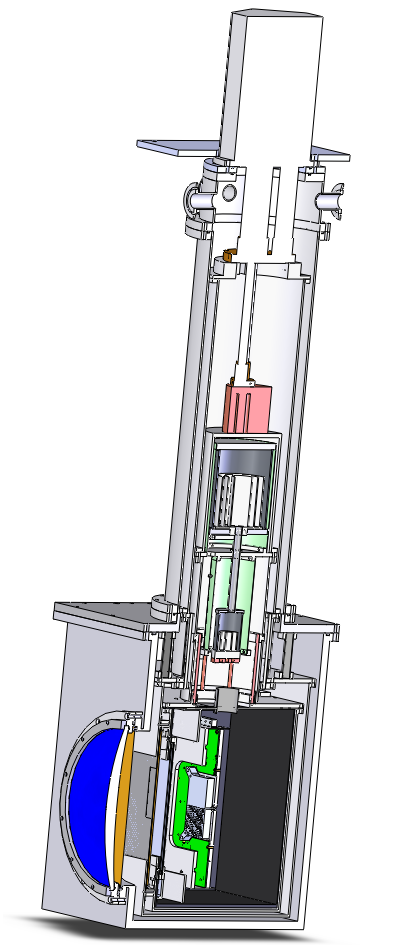
\includegraphics[width=2.6in]{./images/cryostat-cutaway.png}};
    \begin{scope}[x={(image.south east)},y={(image.north west)}]
	    %\draw[help lines,xstep=.1,ystep=.1] (0,0) grid (1.5,1);
		%\foreach \x in {0,1,...,15} { \node [anchor=north] at (\x/10,0) {0.\x}; }
		%\foreach \y in {0,1,...,9} { \node [anchor=east] at (0,\y/10) {0.\y}; }
		
        \draw[red,ultra thick,rounded corners] (0.50,0.7) rectangle (0.85,0.75) node[below left] {\textbf{A}}; % PTC407 1st stage CH
        \draw[red,ultra thick,rounded corners] (0.56,0.595) rectangle (0.71,0.64) node[below left] {\textbf{B}}; % PTC407 2st stage CH
        \draw[red,ultra thick,rounded corners] (0.53,0.55) rectangle (0.78,0.595) node[below left] {\textbf{C}}; % Cu Cylinder
        \draw[red,ultra thick,rounded corners] (0.505,0.32) rectangle (0.75,0.55) node at +(-0.1,-0.03) {\textbf{D}}; % sorp fridge
        \draw[red,ultra thick,rounded corners] (0.4,0.06) rectangle (0.70,0.26) node[red,below left] {\textbf{E}}; % Focal Plane
        
        \draw[thick,<->] (1.05,0.04) -- +(0,0.31) node[midway,right] {18 in}; % scale bar
    \end{scope}
\end{tikzpicture}
\caption{Cutaway view of the \Imager. \textbf{A} PT407 1st stage cold head \textbf{B} PT407 2nd stage cold head \textbf{c} Cu cylinder connected PT407 2\textsupescript{nd} stage cold head to Cu tube, which then connects to \He4-sorption refrigerator condensation plate. \textbf{D} \He4-sorption refrigerator \textbf{E} Focal Plane. Copper ropes connecting focal plane to 1~K cold plate are not visible in this view.}
\label{fig:cryo-cutaway}
\end{figure*}

\begin{table*}[t]
\centering
\caption{Temperatures Reached Under Optical Load xxx should I add temps when closed optically?}
\label{tab:temp-optical-load}
\begin{tabular}{l r}
\toprule
Temperature Stage &  Temperature (K)\\
\midrule
PTC 1st Stage Cold Head 			& 48 \\
PTC 2st Stage Cold Head 			& 3.5 \\
Cryostat ``50 K'' Cold Plate 		& 84 \\
Cryostat ``4 K'' Cold Plate 			& 5.8 \\
Sorption Fridge Condensation Plate 	& 3.7 \\
Focal Plane 						& 0.962 \\
\bottomrule
\end{tabular}
\end{table*}

Options for reaching temperatures below the $\sim$1.2~K transition temperature of our \TES\ detectors include: dilution refrigerators, adiabatic magnetization refrigerators, pumped \He4 baths, and \He3- and/or \He4-sorption refrigerators.
We chose a \He4-sorption fridge because of its low cost, ease of operation compared to other solutions, and the fact that the typical base temperatures under no load of $\sim$700~mK is well-matched to our application. xxx actually the key point is temperature - others are in addition.
A  \He4-sorption fridge works by using a charcoal adsorber to pump on a bath of liquid \He4, reducing the \He4 boiling point and thus the temperature of the bath.
The \He4 is contained withing a sealed reservoir so that the refrigerator acts as a closed system requiring no \He4 replenishment. 
While \He4-sorption fridges are commercially available, our team choose to design and build a custom fridge based on a design that has been proven in astronomical applications\cite{devlin_high_2004}.

\figref{fig:he4sorp} shows a schematic depiction of the \Imager's \He4-sorption refrigerator.
The entire refrigerator is filled with 2.07~moles of \He4 gas, giving a pressure of 900~psi at room temperature.
In normal operation the heat switch between the charcoal pumping chamber (``pump'') and the \He4 condensation plate is closed, keeping the charcoal as cold as possible in order to adsorb as much \He4 as possible, keeping the temperature of the cold plate as low as possible.

\begin{figure*}[th]
\centering
\begin{tikzpicture}
    \node[anchor=south west,inner sep=0] (image) at (0,0) {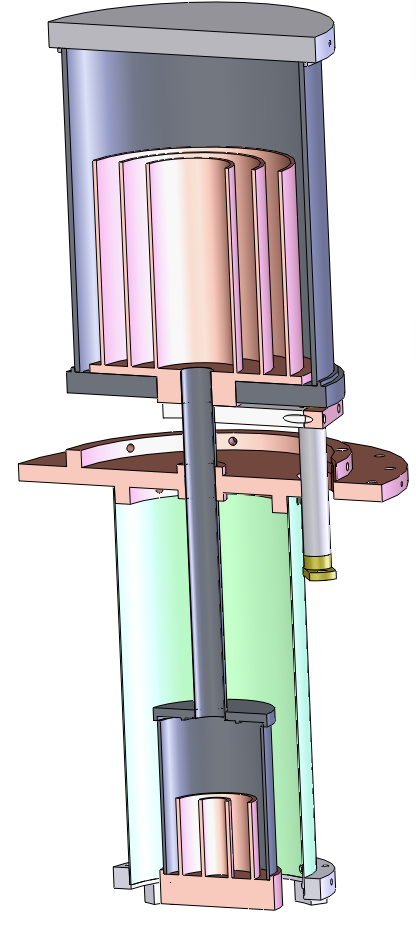
\includegraphics[width=3.0in]{./images/he4-sorp-fridge-cutaway.png}};
    \begin{scope}[x={(image.south east)},y={(image.north west)}]
	    %\draw[help lines,xstep=.1,ystep=.1] (0,0) grid (1.5,1);
		%\foreach \x in {0,1,...,15} { \node [anchor=north] at (\x/10,0) {0.\x}; }
		%\foreach \y in {0,1,...,9} { \node [anchor=east] at (0,\y/10) {0.\y}; }
        \draw[blue,ultra thick,rounded corners] (0.10,0.56) rectangle (0.86,1.01) node[below left] {\textbf{A}}; % pump
        \draw[blue,ultra thick,rounded corners] (0.02,0.56) rectangle (1.03,0.44) node[above left] {\textbf{B}}; % cond plate
        \draw[blue,ultra thick,rounded corners] (0.70,0.56) rectangle (0.88,0.36) node[above left] {\textbf{C}}; % heat switch
        \draw[blue,ultra thick,rounded corners] (0.35,0.25) rectangle (0.72,-0.02) node[above left] {\textbf{D}}; % pot
        
		\draw[thick,<->] (0.9,0.02) -- ++(0,0.21875) node[midway,right] {3 in}; % scale bar
    \end{scope}
\end{tikzpicture}
\caption{Cutaway view of the \He4-sorption refrigerator. \textbf{A} Charcoal pumping chamber (``pump''). The charcoal is attached to the concentric copper cylinders. Cylinders are used to maximize the surface area covered by the charcoal. \textbf{B} Condensation plate. This copper plate is kept below the boiling point of \He4 in order to provide a point in the refrigerator for \He4 to condense and drip into the condensation pot. \textbf{C} \He4 gas gap heat switch. This heat switch is used to cool the charcoal in order to pump on the \He4 bath in the condensation pot. \textbf{B} \He4 condensation pot (``pot''). The condensed \He4 accumulates here. The concentric cylinders provide additional surface area for thermal contact to the liquid \He4. Not shown is a small (xxx check size from Bob) constriction in the stainless steel tube connecting the pump and pot, intended to restrict the flow of superfluid \He4 away from the pot.}
\label{fig:he4sorp}
\end{figure*}

Cycling the refrigerator requires four steps.
First the heat switch is opened.
The \He4-sorption refrigerator uses a \He4 gas-gap heat switch manufactured by Chase Cryogenics\footnote{Chase Research Cryogenics, Ltd. Sheffield, UK}, which requires 5 minutes of waiting time in order for the switch to fully open.
Second, the pump is heated by applying \SI{5}{\W} via a \SI{500}{\ohm} power resistor.
This power is applied until the temperature of the pump reaches 40 K, which is high enough to drive nearly all of the adsorbed \He4 off of the charcoal.
Third, the power to the pump is turned off.
Once the temperature of the condensation plate falls below the boiling point of \He4, \He4 will begin to condense on its walls, dripping into the \He4 condensation pot (``pot'').
Fourth, once the temperature of the pot has fallen to 4.0~K, the heat switch is turned back on.
This cools the pump, allowing \He4 to again adsorb onto the charcoal, which has the effect of pumping strongly on the pot, and cooling the \He4 contained there to the base temperature of $\sim$ 970~mK under optical load.
This process is easy to automate, and a LabView program cycles the fridge automatically every night while the system is operating.

Under optical load, a full cycle of the \He4-sorption refrigerator takes approximately 4 hours, reaching a base temperature of $\sim$~970~mK.
When no additional load is applied the hold time is 9 hours.
When the temperature of the stage is held at the typical operating temperature of 1100~mK the hold time is only 3:45 hours.

\tableref{tab:fp-thermal-load} shows the predicted heat load on the \He4-sorption refrigerator.
It excludes parasitic load inherent to the sorption refrigerator itself. xxx mention parasitic load here?

xxx - include data on temp vs load for the fridge?

\begin{table*}[ht]
\centering
\caption{Predicted Thermal Load on 1~K Stage. These calculations assume that the readout wiring and Ti-6Al-4V spiders are running from 6.4~K to 1.0~K.}
\label{tab:fp-thermal-load}
\begin{tabular}{@{}lrr@{}}
\toprule
 & \multicolumn{2}{c}{Predicted Thermal Load} \\
\cmidrule(r){2-3}
Heat Load Source & 1004 Detectors (\si{\uW}) &  251 Detectors (\si{\uW}) \\
\midrule
Readout wiring 								& 50 & 125 \\
Series array \SQUID\ modules 		& xxx & xxx \\
\SQUID\ multiplexing chips 				& xxx & xxx \\
Detectors shunt resistors 			& 5 & 18 \\
Detectors (Optical + Electrical)		& 0.25 & 1 \\
Ti-6Al-4V spiders 							& 130 & 130 \\
Out-of-band optical power 			& xxx & xxx \\
\midrule
Total												& 185 + xxx & 274 + xxx \\
\bottomrule
\end{tabular}
\end{table*}

\section{Optical Design}\label{s:optical-design}

% xxx diagram like fig 4in schwan2011 would be good

\section{Feedhorn Design}\label{s:feedhorn-design}

% xxx where do I explain the choice of a square grid? Ans: section 6.3
% xxx where do I explain the missing 20 detectors?

Millimeter and submillimeter astronomical instruments using \TES\ detectors use many different strategies for coupling light onto detectors: filled arrays of absorbers\cite{swetz_overview_2011,holland_scuba-2:_2013}, antennas with lenslets\cite{keating_ultra_2011}, phased antenna arrays\cite{obrient_antenna-coupled_2012}, corrugated feedhorns \cite{austermann_sptpol:_2012,niemack_actpol:_2010}, and smooth-walled conical feedhorns \cite{schwan_invited_2011,spt}.
The \Imager\ uses smooth-walled feedhorns because they are easy to design and easy to machine.
Smooth-walled feedhorns do not have the nice polarization properties of corrugated feedhorns \cite{clarricoats_corrugated_1984}, but this is not a concern here because the \Imager\ is polarization-insensitive.

\figref{fig:feedhorn-parms} depicts a smooth-walled conical feedhorn and its interaction with the optical system.
As discussed in section \sectionref{s:optical-design}, although the optical system has a secondary mirror as well, for many purposes the secondary mirror can be ignored and the system treated as a system of feedhorns illuminating only a primary mirror with a hole in its center.
If a feedhorn is observing a temperature distribution $T_{target}(\theta,\phi)$, and is pointed in a direction $(\theta_0, \phi_0)$, then the temperature observed by the feedhorn will be
\begin{equation}
    T_{eff}(\theta_0,\phi_0) = \int \, d \Omega \, T_{target}(\theta - \theta_0,\phi - \phi_0) P(\theta,\phi).
\end{equation}
The function $P$ is called the ``beam'' or ``beam pattern'' of the feedhorn, and describes the pattern of radiation to which the feedhorn is sensitive.
Although the \Imager\ is always receiving radiation, never transmitting, this thesis often writes about the beam pattern as if it were transmitting radiation, e.g.\ in decribing the portion of the ``beam'' that strikes the primary mirror.
This is acceptable because the transmitting and receiving beam patterns are exactly the same\footnote{This is a consequence of the reciprocity relationships obeyed by the Maxwell equations. See, e.g.\ \cite{balanis_antenna_2005} for a detailed explanation.}.
When using this expression one must keep in mind that the fraction of the beam that spills off the primary mirror (e.g.\ the unshaded region in \figref{fig:feedhorn-parms}) will see not the temperature distribution of the target, but a temperature distribution determined by what is beyond the primary mirror\footnote{Because of the presence of the secondary mirror, some of this temperature distribution will be in front of the system, and some will be behind.}.
The fraction of the beam that strikes the primary mirror and proceeds to the target is called the spillover efficiency $\eta_s$.

\begin{figure*}
\centering
\includegraphics{drawings/ch4-feedhorn-parms.pdf}
\caption{Schematic showing important parameters of a feedhorn and its beam. The beam appears to emerge from the phase center, a distance $l_c$ behind the mouth of the feedhorn in this diagram. The main lobe of the beam is approximated well by a Gaussian, here characterized by a full-width-half-maximum (\FWHM) beam width. The shaded fraction of the Gaussian represents the part of the beam that falls onto the primary mirror and reaches the target.}
\label{fig:feedhorn-parms}
\end{figure*}

The feedhorn opening diameter $D$ is chosen to minimize the total \NETD\ of the system.
The total \NETD\ was given in \sectionref{xxx} as
\begin{equation}
    NETD = \frac{NEP_{tot}}{2 k_B \Delta \nu \eta_{tot} \sqrt{2 \tau}}.
\end{equation}
To make the factors depending on the size of the feedhorns more clear we can break the optical efficiency $\eta_{tot}$ into a product of two factors, $\eta_s$ and $\eta_{other} = \eta_{tot} / \eta_s$.
We then note that the integration time per pixel $\tau$ is inversely proportional to the number of detectors $N$.
This leads to
\begin{equation}
    NETD \propto \frac{NEP_{tot}\sqrt{N}}{\eta_s}.
\end{equation}

The critical relationship is that as a feedhorn's opening diameter increases, the width of the beam becomes smaller.
Small beam angles increase $\eta_s$, which improves \NETD.
However, the diffraction-limited area on the focal plane that can be covered by feedhorns is fixed, so that increases the horn opening diameter reduces the number of detectors $N$, which worsens \NETD.
Choosing an optimal feedhorn size requires trading these two effect off against each other to minimize \NETD.

There are four additional factors to consider.
First, $NEP_{tot}$ is not neccesarily independent of $\eta_s$.
In a detector-noise limited system it will be, but in a system that is photon-noise-limted, $NEP_{tot}$ may worsen, stay the same, or improve, depending on the temperature seen by the spilled over portion of the beam.
Indoors all of the beam will see roughly the same temperature as the target, so that total photon noise will stay the same.
Outdoors the situation is more complicated because the temperature seen by the spilled over beam will depend on the local scenery and weather conditions.
For simplicity, the analysis of optimum feedhorn size in this chaper made the assumption that the noise seen by a detector is independent of the beam size.

Second, for a Cassegrain optical system, $\eta_s$ is not a monotonic function of $D$.
The secondary mirror obstructs the central part of the beam, preventing it from reaching the target.
This means that narrow beams can have poor $\eta_s$ because a large fraction of the main lobe of the beam will be blocked.

Third, the choie of readout system and wiring places a firm upper limit on the number of detectors in the system of 1024.
Fourth, the dependence of the number of detectors $N$ on the feedhorn diameter $D$ is not a smooth function, because it is not possible to have, e.g., 1/3 of a feedhorn.
As explained in \sectionref{xxx6.3}, the \Imager's detectors are laid out on a square grid.
So it is more helpful to think of the feedhorn diameter as a value that can take on a discrete set of values that depends on the number of feedhorns per each side of the grid.

A \MATLAB\ program was used to find the optimum feedhorn size.
The program uses an analytic expression for the beam pattern developed in \cite{green_radiation_2006,narasimhan_modes_1971,}.
The far-field electric field pattern takes the form
\begin{equation}
    \vect{E}(\theta,\phi) = E_{\theta} \sin{\phi} \hat{\theta} + E_{\phi}(\theta) \cos{\phi} \cos{\theta} \hat{\phi}.
\end{equation}
Here $E_{\theta}$ and $E_{\phi}$ are functions depending the horn diameter $D$ and opening half-angle $\alpha$, and involving definite integrals of Bessel functions, not reproduced here.
This expression is for the waveguide mode polarized along the $\pi/2$ direction.
The \Imager's detectors are unpolarized, so detect both waveguide polarizations equally (see \sectionref{xxx} for confirmation of this via simulations).
The total power beam map is thus given by the incoherant sum
\begin{equation}
    P(\theta, \phi) = (|\vect{E}(\theta, \phi)|^2 + |\vect{E}(\theta, \phi+\pi/2)|^2,
\end{equation}
which simplifies to 
\begin{equation}
    P(\theta) = |E_{\theta}(\theta)|^2 + |E_{\phi}(\theta)|^2 \cos{\theta}^2,
\end{equation}
which is independent of $\phi$, as expected for an unpolarized detector.

To calculate the spillover efficiency of an individual feedhorn, the \MATLAB\ program integrates $P$ over the angles $\theta$ that illuminate the primary mirror and reach the target: \SIrange{5.3}{13.6}{\degree}\footnote{see \sectionref{s:optical-design}}.
\figref{fig:spill-vs-alpha-diam} shows a contour plot of spillover efficiency as a function of $D$ and $\alpha$.
The blue asterisk matches the parameters for the feedhorns chosen for the \Imager.
This plot makes it clear that $\eta_s$ depends much more strongly on $D$ than on $\alpha$.
$\alpha = \SI{9.4}{\degree}$ was chosen as a value that is easy to machine, keeps the thermal mass of the feedhorn array relatively low (small values of $\alpha$ lead to long feedhorns and higher thermal mass), and it not too far from the maximum achievable $\eta_s$ for any fixed feedhorn diameter $D$.

\begin{figure*}[th]
\centering
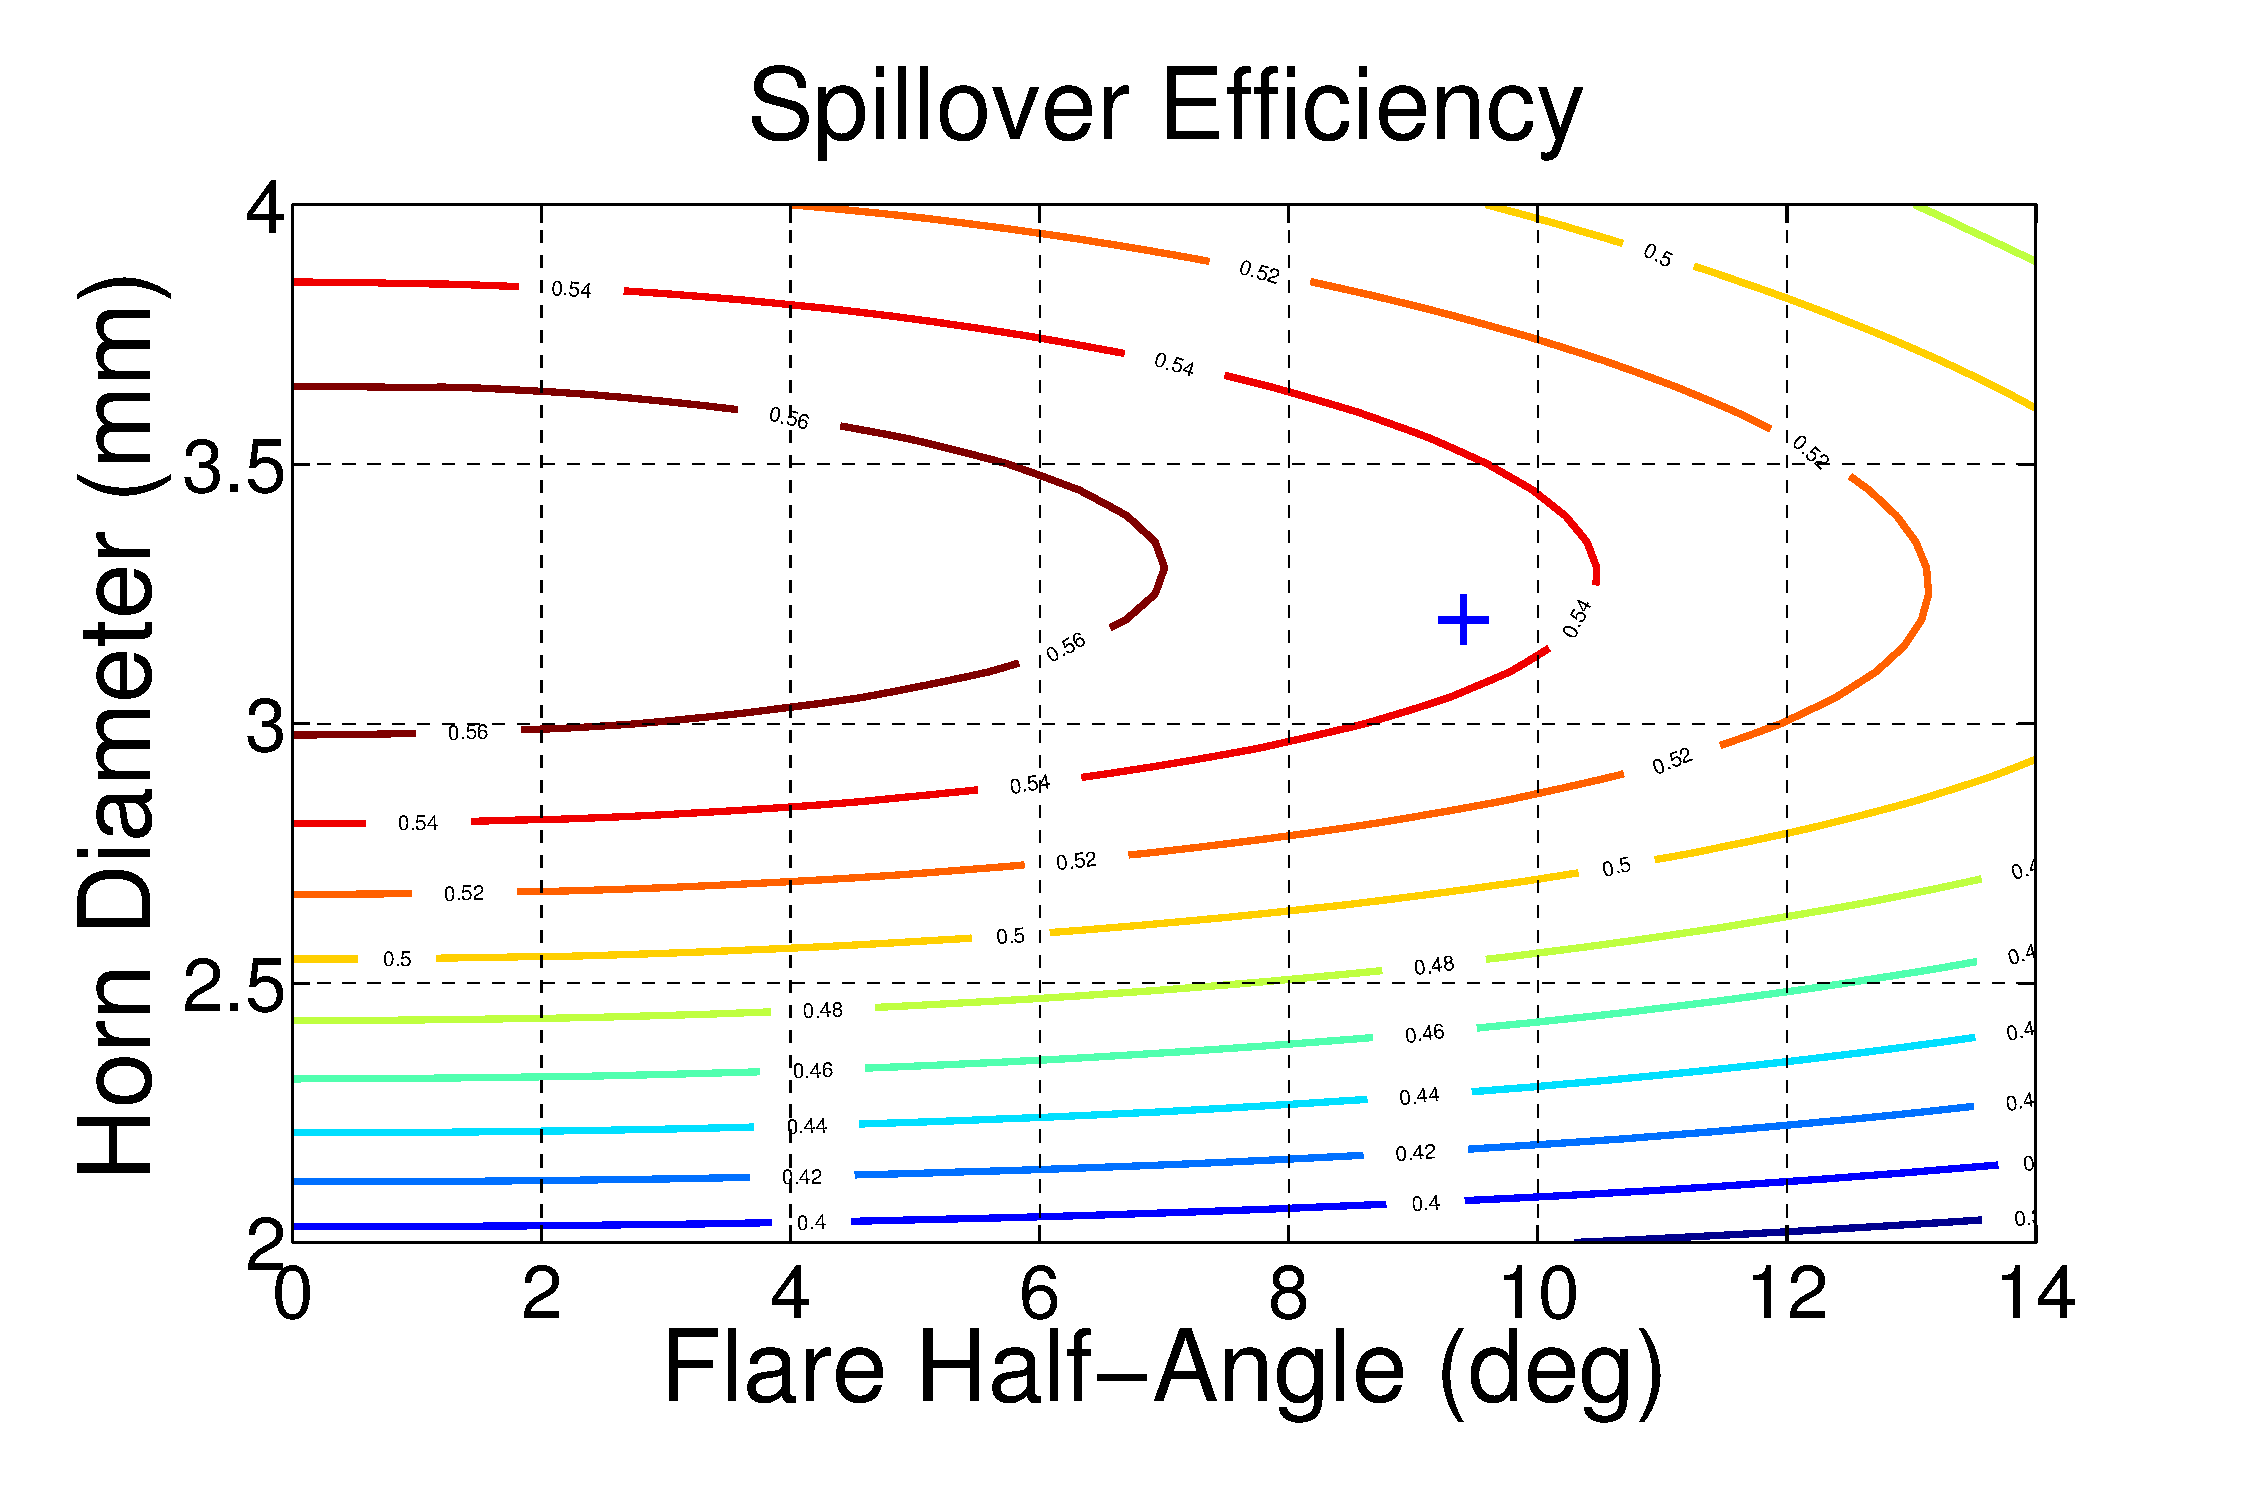
\includegraphics[width=3.0in]{./images/spill_vs_alpha_diam.pdf}
\caption{Plot showing feedhorn spillover efficiency $\eta_s$ as a function of horn diameter $D$ and horn flare half-angle $\alpha$. The blue asterisk shows the feedhorn parameters used in the \Imager. xxx need to replace with version that has * sign at real feedhorn values!}
\label{fig:spill-vs-alpha-diam}
\end{figure*}

The feedhorn diameter chosen does not maximize $\eta_s$, because it turned out that a smaller \NETD\ could be achieved by using a larger number of smaller feedhorns.
In fact, as \figref{fig:netd-num-feeds} shows, an even larger number of even smaller feedhorns is predicted to reduce \NETD\ by xxx \%.
However, as mentiond above, the maximum number of detectors that can be readout by our system is 1024, so $D = xxx$ was chosen as the optimal feedhorn diameter.

\begin{figure*}[th]
\centering
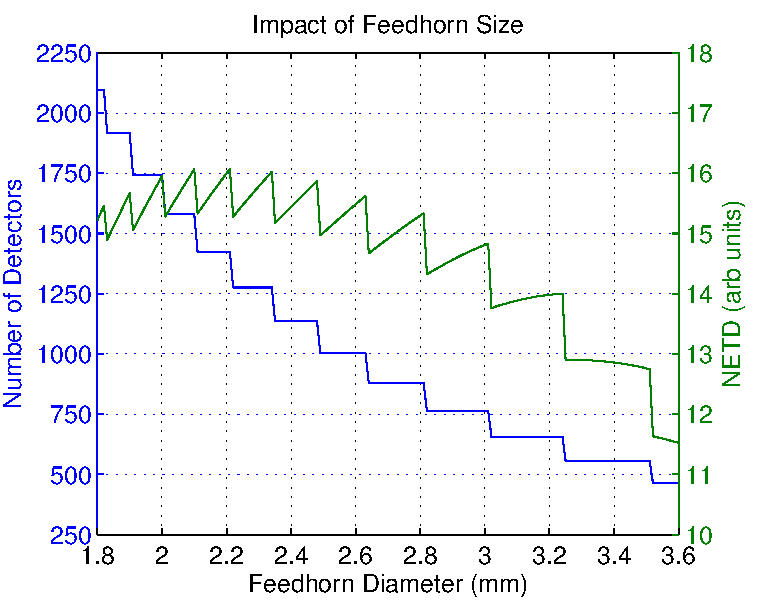
\includegraphics[width=3.0in]{./images/netd_num_feeds.pdf}
\caption{Plot showing how total number of detectors and system \NETD\ depend on diameter chosen for feedhorns. The number of detectors is a discrete function of the feedhorn diameter because it is not possible to have a fractional part of a feedhorn. \NETD\ is maximized with xxx feedhorns of diameter xxx, but the \Imager\ uses 1004 feedhorns of diameter xxx because of readout limitations. xxx Is this plot right? I chose 2.68 mm (cold), which leads to ~800 detectors, not 1024.}
\label{fig:netd-num-feeds}
\end{figure*}

xxx - show that beam is well-approximated by a gaussian over the area of the primary mirror.

%\subsection{Far-field beam pattern and system spatial resolution}
%
%A Fourier transform relationship exists between the electric field illuminating the aperture of an optical system and the electric field far away form the aperture\cite{xxx}.
%\[
%   xxx write the expression here,
%\]


\section{Acknowledgments}

Bob Schwall and William Duncan of NIST designed the cryostat/mirror mount and the \He4 sorption refrigerator.
The refrigerator was filled with \He4 by Simon Dicker at the University of Pennsylvania.
Bob Schwall of NIST designed the cryostat, and provided useful advice and help in the lab during commissioning of the cryostat.
William Duncan designed, procured, and assembled the optical system.
Mandana Amiri and Matthew Hasselfield provided extensive, timely and invaluable support for the MCE hardware and software.


% \chapter{Detector Design}\label{c:det-design}

% \chapter{Focal Plane Design}\label{c:fp-design}

% \chapter{Prototype Detector Characterization}\label{c:proto-det}

%%%\chapter{Subarray Characterization}\label{c:det-array}

The detectors in the first 251-detector subarray have not all been characterized to the same extent.
Partly this is due to manpower and time constraints.
Additionally, as described in \sectionref{sec:g-psat}, the saturation power of the detectors is \abt 2 times higher than expected, which means that only some detectors be driven normal, and only at bath temperatures very close to $T_c$.
In particular, none of the detectors can be driven normal at the operating bath temperature for the array of 1100~mK.
This means that we do not have \IV\ curves for any detectors at operating conditions, which limits the characterization than can be performed.

Seven detectors used in taking images have working heaters and no other problems.
These heaters allow us to take full \IV\ curves at all bath temperatures, allowing estimate of the detector thermal conductance $G$.
The heaters also allow a direct measurement of detector responsivity and time constants, and thus allow a measurement of detector noise referred to optical power incident on the detector.
These later measurements have been carried out on four of the seven detectors.
Additionally, \Loop, $\beta_I$ and $R$ at operating conditions have been measured for all working detectors.
This chapter describes all these measurements, as well as measurements of shunt resistors and inductors for all detectors.
\tableref{tab:measurements} summarizes all of the measurement that have been performed and described in this chapter.
Sections discussing common mode noise, microphonic pickup and noise aliasing are also included.

Note that this lack of detector characterization does not prevent the array from working.
It merely limits our understanding of the behavior of the detectors.
A more detailed characterization of more detectors will be carried out prior to fabrication of any additional arrays.

\begin{table*}[t]
\centering
\caption{Summary of measurements made on first 251-detector subarray}
\label{tab:measurements}
\begin{tabular}{l l l}
\toprule
Measurement &  Section & Which Detectors  \\
  \midrule
Choice of Optimal \MCE\ servo gain parameters & \ref{sec:mce-servo-gain} & All columns \\
$R_{sh}$ and $L_{ny}$ & \ref{sec:shunt-nyquist} & All working detectors \\
Heater Resistors & \ref{sec:heater-r} & Seven detectors with good heaters on column 0 and 1 \\
$\tau$ & \ref{sec:tau-nat} & Four detectors with good heaters on column 0 \\
$G$, $T_c$, $n$, $P_{sat}$ & \ref{sec:g-psat} & Seven detectors with good heaters on column 0 and 1 \\
$\tau_{eff}$ and \DC\ responsivity & \ref{sec:teff-resp} & Seven detectors with good heaters on column 0 and 1 \\
\Loop, $\beta_I$, $R$ at a range of bias points & \ref{sec:bias-step} & Seven detectors with good heaters on column 0 and 1 \\
\Loop, $\beta_I$, $R$ at standard operating conditions & \ref{sec:bias-step} & All working detectors\\
Detector noise at a range of bias points & \ref{sec:det-noise} & Four detectors with good heaters on column 0 and 1 \\
\bottomrule
\end{tabular}
\end{table*}


\section{Choice of \textsc{MCE} Servo Gain Parameters}\label{sec:mce-servo-gain}

As described in \sectionref{sec:det-readout}, the \MCE\ operates the \SQUID\ multiplexing system.
It supports extensive configuration options ranging from \SQUID\ bias current values to multiplexing speed, to the order in which rows should be reported to client software \cite{_mcewiki_2014}.
This thesis does not describe the process of choosing most of these parameters.
The one exception is the choice of \PID\ parameters for the flux-locked-loop servo that linearizes the output of the \SQUID\ amplifier chain.
This section describes the choice of these parameters for different readout situations.

The feedback applied to an \SQ1 during frame $n+1$ is defined as \cite{mce_team_data_2013}
\begin{equation}
  FB_{n+1} = \frac{1}{2^{12}} \left[P q_n + I \sum_{i=1}^n e_i + D (e_n - e_{n-1}) \right].
\end{equation}
Here $e_n$ is the error observed during frame $n$, $q_n \equiv e_n + b q_n$ (where $b$ is some number small than 1), and $P$, $I$, and $D$ are the proportional, integral, and derivative terms of the \PID\ loop, respectively.
The $FB$ values are expressed in terms of \DAC\ counter units applied to the \SQ1 feedback, and the errors $e$ are in terms of \ADC\ values for the output of the readout chain.
The \Imager\ is operated with $P = D = 0$, so that the feedback simplifies to
\begin{equation} \label{eqn:mce-pid-i-only}
  FB_{n+1} = \frac{I}{2^{12}} \sum_{i=1}^n e_i.
\end{equation}

Using only $I$, the \MCE\ servo loop acts like a 1-pole filter.
Higher values of $I$ increase the bandwidth of this filter until a ``critical gain'' is reached, as which point the feedback loop becomes unstable and begins to oscillate.
$I$ should be chosen so that the bandwidth of this filter is greater than that of the detectors themselves, but $I$ should not approach the critical gain too closely.

The servo $I$ parameter was chosen to minimize \SQUID\ noise and allow sufficient bandwidth to readout the full bandwidth of the detectors.
The target servo bandwidth depends on the measurement being made.
When operating the array in normal conditions, the data readout rate is either \SI{3125}{Hz} or \SI{3030.3}{Hz}, depending on whether the dark \SQUID\ is read out.
The time constant for the associated Nyquist frequencies are \abt~\SI{0.1}{ms}, so there is no need to use $I$ values with more bandwidth than this\footnote{Doing so is counter-productive, because it will alias \SQUID\ noise into the detector band}.
Electrical detector time constants are \abt~\SI{4}{ms} in the superconducting state, and \abt~\SI{0.14}{ms} in the normal state.
While biased into the transition, $\tau_{eff}$ is in the range \SIrange{1}{4}{ms}.
\figref{fig:ch8-servo-tau-est} shows the impact of the servo rolloff on estimation of time constants from single-pole response functions.
To reduce the error in the estimated time constant below \SI{2}{\percent}, the servo time constant should be below \SI{5}{\percent} of the time constant to be measured.
This criteria corresponds to \SI{2e-4}{s} for the superconducting state and as fast as \SI{5e-5}{s} for detectors operating in the transition.

\begin{figure*}
\includegraphics{drawings/ch8-servo-tau-est.pdf}
\caption{Plots summarizing requirements on $\tau_{servo}$ for accurate measurements of detector time constants.
\textbf{Left} Plot showing exact response to step function of a detector with $\tau = \SI{4}{ms}$, the response as filtered by a servo with $\tau_{servo} = \SI{1}{ms}$, and the best fit to the filtered response. The estimated $\tau$ is \SI{23}{\percent} too high.
\textbf{Right} Plot showing fraction overestimate of $\tau$ vs. relative size of $\tau_{servo}$.
For less than \SI{2}{\percent} error, $\tau_{servo}/\tau < \num{0.05}$ is required.
}
\label{fig:ch8-servo-tau-est}
\end{figure*}

Measuring the bandwidth of the servo loop is challenging because when the detectors are in the superconducting state the Johnson noise of the shunt resistor is higher than the \SQUID\ noise and the Johnson noise rolloff is \abt \SI{4}{\ms}, both factors which make it difficult to identify the servo rolloff from power spectra.
However, if the bath temperature is raised above $T_c$ for the Al wirebonds connecting the \TES\ circuit to the input coils of the 1st stage \SQUIDs, the total resistance of the \TES\ circuit is raised from \SI{150}{\uohm} to \SIrange{20}{50}{\mohm}.
This high resistance drives the Johnson noise of the load resistor below the \SQUID\ noise, and pushes the $L/R$ rolloff of the Johnson noise to \SI{3e-5}{s} or faster (\SI{3}{\dB} frequency of \SI{5}{\kilo\Hz} or higher), making a measurement of the servo bandwidth much easier.

To choose $I$ values, I acquired data at the fastest multiplexing rate possible for 33 rows\footnote{This rate is achieved by only reporting one of the eight columns to the readout computer. The limiting factor in how fast the entire array can be multiplexed is packaging and sending the data to the readout computer.}, \SI{15151.5}{Hz} while the system was at a temperature of \SI{1.3}{\K}.
For every row and column that has a detector that responds in the superconducting state, I fit the resulting noise power spectrum to an equation of the form
\begin{equation}
  \frac{N_{SQ}}{1 + (2 \pi \tau_{servo})^2},
\end{equation}
Where $N_{SQ}$ is the white noise level and $\tau_{servo}$ gives the bandwidth of the servo loop.

\figref{fig:ch8-servo} shows the resulting white noise levels and $\tau_{servo}$ values for a range of servo gain values $I$.
The \SQUID\ white noise level is higher when operating with negative $I$ values, so we have chosen to use positive $I$ values.
When measuring time constants $I=50$ has been used for all columns, to maximize the number of detectors below the $\tau_{servo} =$ \SIrange{2e-4}{5e-5}{s} range.
This also places most detectors in a region where \SQUID\ noise will be aliased into the measurement band, but because I always average over many measurements, this is not a major concern.

For taking video images, the servo does not need to be run as aggressively.
As shown in \figref{fig:ch8-teff-si-pred}, most detectors have $\tau_{eff}$ right around \SI{1.25}{\ms}, with only a few slower than this.
A servo gain of 20 puts $\tau_{servo}$ below \SI{0.6}{\ms} for all detectors, so there is no need to operate at a higher servo gain when taking video images.
Even operating with a servo gain of 10 puts \SI{95}{\percent} of the $\tau_{servo}$ below \SI{1}{\ms}, so operating at a servo gain of 10 is also acceptable, though not as ideal as 20.

\begin{figure*}
\includegraphics{drawings/ch8-servo.pdf}
\caption{Plots summarizing behavior using different servo gains $I$.
  Box plot boxes represent the \SIrange{5}{95}{\percent} quantiles, middle line the median, upper and lower whiskers the maximum/minimum values, across all rows/columns with detectors that respond in the superconducting state.
\textbf{Upper} Plot of \SQUID\ $\tau_{servo}$ vs servo gain $I$.
Servo bandwidth increases with $I$.
At $I \ge \num{60}$, very small $\tau_{servo}$ begin to appear. This indicates either a rolloff above the bandwidth of the measurement, or the beginning of an unstable servo loop.
The few high $\tau_{servo}$ values at gains of 80 and 100 are a result of the fitting routine failing, probably due to an unstable servo loop.
\textbf{Lower Left} Close-up view of upper plot for gains from 10 to 50.
\textbf{Lower Right} Plot of median \SQUID\ white noise level vs. servo gain $I$. Positive gains consistently give lower dark \SQUID\ noise levels.
}
\label{fig:ch8-servo}
\end{figure*}

\section{Shunt Resistance Measurements}\label{sec:shunt-nyquist}

Our shunt resistors are located on interface chips that contain both shunt resistors and Nyquist inductors.
The specific chips used were extra chips leftover from the ABS\cite{kusaka_modulation_2013} project.
The design resistance of the shunts was \SI{180}{\uohm}, and the design inductance was 609~nH\footnote{John Appel, personal communication}.
Each chips contains 32 shunt resistors and 32 inductors.

To measure $R_{sh}$ and $L$ for these chips I took noise measurements using zero detector bias current at two different bath temperature: 980~mK and 1160~mK.
At these bath temperatures and at zero detector bias the detectors are superconducting, so that measured noise is due to the shunt resistor, any parasitic resistance, and SQUID noise in the multiplexed readout system itself.
Data was collected at 3030.3~Hz, and 20 data acquisitions lasting 33 seconds were taken at each bath temperature.

A power spectrum was estimated for each detector for each data acquisition using \MATLAB's \texttt{pwelch} function, using a \FFT\ size of $2^{12}$.
Each resulting power spectrum was fit to a function of the form
\begin{eqnarray}\label{eqn:scnoise-fit}
	\frac{4 k_B T_b}{R_{sh}} \frac{1}{1 + (2 \pi f (L/R_{sh}))^2} + SQ,
\end{eqnarray}
where $k_B$ is Boltzmann's constant, $T_b$ is the bath temperature for the measurement, and $f$ is the frequency.
The shunt resistance $R_{sh}$, inductance $L$, and readout chain white noise level $SQ$ are the values extracted from the fit.

\figref{fig:rsh-l-plots} shows histogram plots of the resulting \Rsh\ and $L$ values.
\Rsh\ has a mean of \SI{149}{\uohm} with standard deviation \SI{6}{\uohm}.
The measured value for \Rsh\ also includes any parasitic resistance in the circuit, but no evidence for significant parasitic resistance has ever been seen, so this parasitic resistance is assumed to be zero.

The measured value for $L$ includes the Nyquist inductance on the interface chip, the input inductance of the first-stage \SQUID\ of the multiplexed readout system, as well as any parasitic inductance in the circuit.
Using this measurement it is not possible to extract the inductance of the Nyquist induct-or itself, but this is not a problem because the total inductance is the relevant  quantity for understanding the behavior of the detector and its circuit.

$L$ has a mean of 568~nH with a standard deviation of 86~nH.
However, this mean includes two sets of clear outliers: all values for multiplexing row 4 are clustered around 200~nH, and all values for multiplexing row 25 are clustered around 440~nH.
The reason for these low inductances is not understood.
Excluding rows 4 and 25,  $L$ has a mean of 587~nH with a standard deviation of 44~nH.

The outlier $L$ values are more clearly visible in the lower left plot in \figref{fig:rsh-l-plots}, which also shows a small correlation between \Rsh\ and $L$.
It is not known whether this correlation is a real physical effect or an artifact of the measurement process.

\begin{figure*}
\includegraphics{drawings/ch8-rsh-l-plots.pdf}
\caption{Plots summarizing results of measurements of shunts and Nyquist inductors.
\textbf{Upper Left} Histogram of shunt resistance \Rsh.
\textbf{Upper Right} Histogram of total inductance in circuit, which includes the interface chip Nyquist inductor, the inductance of the SQ1 input coil, and any parasitic inductance.
\textbf{Lower Left} Scatterplot showing all measured Rsh and L values. A correlation is apparent, the reason for which is not understood.
\textbf{Lower Right} Plot showing current noise power spectrum extracted from a single data acquisition for \RCm{20}{6}, along with predicted power spectrum based on best fit to \eqnref{eqn:scnoise-fit} across all data acquisitions. The best fit values are $\Rsh=\SI{155}{\uohm}$, $L = \SI{616}{nH}$, and \SQUID\ white noise level of \Inoise{1.2e-10}.}
\label{fig:rsh-l-plots}
\end{figure*}

\section{Measurement of Heater Resistors} \label{sec:heater-r}

Thirty-one detectors have heater resistors connected to bond pads.
Twenty-three of these have the heaters wired to the heater bias line.
Of these 23, there are nine detectors which show no response to applied heater power.
Five of these nine are on the cut list (see \sectionref{sec:ch9-det-cuts}), so this is not surprising.
But four detectors can be biased into the transition and work well, but show no response to applied heater power (\RC{4}{7}, \RC{5}{7}, \RC{6}{6}, \RC{7}{6}).
The reasons for these detectors not showing a response to heater power are not fully understood.
This leaves 14 working detectors that also show a response to applied heater power.
However, a short between one of the \TES\ bias lines and the heater bias line means that ramping the current bias for some of the \TES\ detectors also ramps the heater bias.
This means that for seven of the 14 working detectors that show a response to applied heater power, interpreting \IV\ curves is difficult because a different amount of heater power is applied at each detector bias value.
This means that for these seven detectors it is not possible to measure $G$ or to calibrate the power being applied by the resistors.

This leaves seven detectors with heaters for which \IV\ curves can be taken, and $G$ measured.
The heaters on these seven detectors can be used to directly measure the detector responsivity, noise referred to input optical power, time constants and thermal conductance $G$.
But all of these measurements require knowing the resistance of the heaters.
This section describes my measurement of the heater resistances.

To measure the heater resistances, I took a set of \IV\ curves at constant bath temperature.
For each \IV\ curve I applied a different heater current, so that a different amount of heater power was applied to the \TES\ for each curve.
The total amount of power flowing through the \TES\ thermal conductance $G$ is then given by
\begin{equation}\label{eqn:tes-ptot}
P_{tot} = K(T^n - T_b^n) = P_{opt} + P_{htr} + I^2 R(T,I),
\end{equation}
where $T$ is the temperature of the \TES, $R$ is the resistance of the \TES, and $I$ is the current flowing through the \TES.
I make the assumption that at the start of the superconducting transition $\beta_I = 0$, i.e.\ the resistance of the \TES\ depends only on the \TES\ temperature, and not on the current through the \TES.
This implies that each time the \TES\ reaches, e.g.\ $0.99R_n$, the temperature of the \TES\ is the same, and therefore $P_{tot}$ will be the same.
A relationship of the following form must therefore hold:
\begin{equation}\label{eqn:rhtr-fit}
P_{J} = (P_{tot} - P_{opt}) - I_{htr}^2 R_{htr}.
\end{equation}
A fit can be made to this function, with the quantities $R_{htr}$ and $P_{x} \equiv P_{tot} - P_{opt}$ to be solved for.

\figref{fig:ch8-heater-r-plots} explains this idea further by a series of plots.
The upper left plot shows the \TES\ \IV\ curves.
The upper right plot shows the same data, but transformed into \TES\ Joule power and \TES\ resistance.
As applied heater current decreases, the Joule power at the start of the transition decreases.
In the lower left, the Joule power at $0.99R_{n}$ is plotted vs applied heater current.
A fit to \eqnref{eqn:rhtr-fit} is also plotted.
Finally, the lower right plot show the $R$ vs $P_J$ plots after the heater power has been added to each curve.
This plot shows that the powers are equalized very high in the transition, where the assumption of Joule power dependent only on \TES\ resistance holds.
It also shows that this assumption breaks down deeper in the transition.

\begin{figure*}
\includegraphics{drawings/ch8-heater-r-plots.pdf}
\caption{Plots heater measurements, for the case of \RCm{29}{1}.
\textbf{Upper Left} \IV\ curves. The \IV\ curves should turn vertical when the detector becomes fully superconducting at zero voltage, but these curves shown a non-infinite slope. The reason for this is that the readout system as configured for these \IV\ curves was unable keep up with the rapid change of current in the superconducting branch.
\textbf{Upper Right} Same data as in upper left plot, but represented in terms of \TES\ Joule power and resistance. As the bias current for the heaters is increased, the curves shift to the left.
\textbf{Lower Left} Measured $P_{J}$ vs heater current at $0.99R_n$, as well as fit to \eqnref{eqn:rhtr-fit}.
\textbf{Lower Right} Same plot as upper right, but the heater power based on $R_{htr} = \SI{23.6}{\ohm}$ has been added to each curve.}
\label{fig:ch8-heater-r-plots}
\end{figure*}

\tableref{tab:basic-det-props} lists all measured heater resistors.
The seven heaters for columns 0 and 1 have a mean of \SI{23.8}{\ohm} with a standard deviation of \SI{0.26}{\ohm}.

It is worth noting that determining the values of $R_{htr}$ requires knowing the current through the heaters.
But because $R_{htr}$ is determined through the power dissipated in the resistor, an incorrect assumption about the current will lead to a an incorrect value of $R_{htr}$ which leaves $I_{htr}^2 R_{htr}$ unchanged.
So whenever the value $R_{htr}$ is used to calculated a power, the power value will be correct even in the face of an incorrect assumption about the current through the heater.

\begin{table*}[t]
\centering
\caption{Basic detector properties.
$P_{opt} = 150$~pW is assumed everywhere.
Uncertainties are 95 \% confidence intervals after marginalizing over other fit parameters, and do not include systematic uncertainties due to the unknown value of $P_{opt}$ or uncertainty in the value of the shunt resistors.
}
\label{tab:basic-det-props}
\begin{tabular}{l l l l l l}
\toprule
Detector &  $R_{htr}$ (\si{\ohm}) & $G$ (\si{\nano\W\per\K}) & $n$ & $T_c$ (mK) & $\tau$ (ms) \\
\RCm{29}{1} & 23.6 & 7.63 $\pm$ 0.08 & 3.52 $\pm$ 0.10 & 1209.4 $\pm$ 0.6 & 8.94 $\pm$ 0.1 \\
\RCm{30}{1} & 23.5 & 7.67 $\pm$ 0.07 & 3.54 $\pm$ 0.09 & 1213.9 $\pm$ 0.6 & 8.82 $\pm$ 0.2 \\
\RCm{31}{1} & 24.3 & 7.78 $\pm$ 0.09 & 3.64 $\pm$ 0.11 & 1214.7 $\pm$ 0.7 & 9.45 $\pm$ 0.1 \\
\RCm{32}{1} & 23.9 & 7.01 $\pm$ 0.43 & 3.18 $\pm$ 0.60 & 1211.6 $\pm$ 3.8 & 10.22 $\pm$ 0.1 \\
\RCm{29}{2} & 23.8 & 7.70 $\pm$ 0.09 & 3.62 $\pm$ 0.11 & 1213.7 $\pm$ 0.7 & 9.01 $\pm$ 0.1 \\
\RCm{31}{2} & 23.6 & 7.32 $\pm$ 0.16 & 3.45 $\pm$ 0.22 & 1211.3 $\pm$ 1.4 & 9.51 $\pm$ 0.1 \\
\RCm{32}{2} & 23.8 & 7.50 $\pm$ 0.27 & 3.74 $\pm$ 0.35 & 1215.6 $\pm$ 2.3 & 10.98 $\pm$ 0.1 \\
\midrule
Mean & 23.8 & 7.52 & 3.53 & 1212.9 & 9.56 \\
\bottomrule
\end{tabular}
\end{table*}

\section{Measurement of Natural Time Constant $\tau$} \label{sec:tau-nat}

%% run thesis/ana_tau_nat.m for results

The approach described in \sectionref{sec:tau-nat-theory} was used to measured the natural time constant tau.
The response to a step-function change in applied heater power was measured while the detectors were at $T_{b} = \SI{1100}{\mK}$.
As described in \sectionref{sec:heater-r} the response to multiple steps was averaged together prior to making a fit.
For each bias point the measured time constant $\tau_{meas}$ and change in \TES\ current $\delta I$ was measured. A fit was then performed to \eqnref{eqn:teff-from-tau}:
\begin{equation} \label{eqn:tau-nat-fit}
  \tau_{meas} = \tau - \tau \mathcal{K} (I_{bias} \delta I).
\end{equation}
In this fit, $\tau_{meas}$ is considered the dependent variable, the product $(I_{bias} \delta I)$ is the independent variable, and both $\tau$ and $\mathcal{K}$ are fit for.

\figref{fig:tau-nat-plots} shows an example of fitting to \eqnref{eqn:tau-nat-fit}, and the measured values of $\tau$ are listed in \tableref{tab:basic-det-props}.

\begin{figure*}
  \centering
\includegraphics{drawings/ch8-tau-nat-plots.pdf}
\caption{
  Plot showing example of fit to \eqnref{eqn:tau-nat-fit}, for \RCm{31}{1}.
  The y-intercept at $I_{bias} \delta I = 0$ gives $\tau$, \SI{9.45}{\ms}.
} 
\label{fig:tau-nat-plots}
\end{figure*}

\section{Measurement of \textsc{TES} $G$} \label{sec:g-psat}

With knowledge of the heater resistances, \IV\ curves can be taken over a wide range of bath temperatures, which enables a measurement of the \TES\ thermal conductance $G$.
Similarly to \sectionref{sec:heater-r}, I took \IV\ curves at bath temperatures ranging from 995~mK -- 1160~mK, while adjusting the applied heater power so that each \IV\ curve had a clear normal branch.
I again used the assumption that high in the transition the \TES\ resistance depends on only the \TES\ temperature, so that the Joule power $P_J$ dissipated in the \TES\ at $0.99R_n$ depends only on the bath temperature $T_b$ and the applied heater power $P_{htr} = I_{htr}^2 R_{htr}$. A fit can then be made to \eqnref{eqn:tes-ptot} in the form
\begin{equation}\label{eqn:g-fit}
P_{htr} + P_J + P_{opt}= \frac{G T_c}{n}\left(1 - \left(\frac{T_b}{T_c}\right)^n\right).
\end{equation}
The parameters to be fit to are $G$, $T_c$, and $n$.

A problem arises because the data described in this section were taken when the cryostat was open, so that $P_{opt}$ was non-zero, with an unknown value.
Because $P_{opt}$ is a simple additive constant, it is not possible to fit for this value unless another constraint (such as the value of $T_c$) is known.
However, the value of $P_{opt}$ can be estimated in two different ways. 
First, the predicted optical load of 165~pW from \sectionref{sec:optical-design} can be used.
Second, optical load on the prototype detectors was estimated to be in the range \SIrange{135}{165}{\pW}.
In this analysis I assume $P_{opt} = 150$~pW, while also showing how different assumptions change the values of  $G$, $T_c$, and $n$.

\tableref{tab:basic-det-props} lists the resulting values for $G$, $T_c$ and $n$.
\figref{fig:heater-g-plots} contains plots summarizing and explaining this data.
The uncertainties in $G$, $T_c$ and $n$ introduced by the unknown value of $P_{opt}$ are different.
$G$'s uncertainty from $P_{opt}$ is about the same size as the statistical uncertainty due to the fit, while $T_c$'s uncertainty from $P_{opt}$ is much larger than the statistical uncertainty.
Both of these uncertainties should be taken into account when predicting measurement of detector noise.
$n$ shows no apparent trend with $P_{opt}$.

\begin{figure*}
\includegraphics{drawings/ch8-g-plots.pdf}
\caption{Plots summarizing results of $G$, $T_c$ and $n$ measurements for seven detectors with good heaters.
All error bars and ellipses are 95 \% confidence intervals for statistical error; any systematic error is not included.
\textbf{Upper Left} Plot showing $P_{sat}$ vs $T_b$ for \RCm{31}{2}, assuming $P_{opt} = \SI{150}{\pW}$.
The red line shows the best fit to \eqnref{eqn:g-fit}.
The data covers 25 temperatures from \SIrange{995}{1160}{\mK}, and 11 different heater biases.
\textbf{Upper Right} Scatter plot showing correlation between $G$ and $n$, as well as error ellipses showing covariance between the estimated $G$ and $n$ vales.
\textbf{Lower Left} Plot showing variation of $G$ for \RCm{31}{2} vs assumed value of $P_{opt}$.
The statistical uncertainty in $G$ for this detector is approximately the same as the systematic uncertainty that results from the estimation of $P_{opt}$.
\textbf{Lower Right} Plot showing variation of $T_c$ for \RCm{31}{2} vs assumed value of $P_{opt}$.
In this case the systematic uncertainty is larger than the statistical uncertainty.
The value of $n$ shows no trend with $P_{opt}$.
} 
\label{fig:heater-g-plots}
\end{figure*}

As discussed in \sectionref{sec:det-parm-choice}, the target $G$ value for these detectors was 3.7~nW/K.
The mean value for the seven measured detectors is 7.52~nW/K, 2.0 times larger than the target.
The reason for this discrepancy is not known.
%thz5 high g - 67 um 
%thz5 high g - 80 um 
%thz4 proto - 40 um

Prediction of detector G noise

xxx - need to account for correlation between G, n, Tc that arises from the fit.
Answer: Also covariance with Tc, which you can account for in noise predictions, but makes little difference.

\section{Direct Measurement of Detector Responsivity and $\tau_{eff}$} \label{sec:teff-resp}

Knowledge of $R_{htr}$ allows a direct measurement of the DC responsivity of $\tau_{eff}$ for the seven detectors with heaters.
Steps in heater bias current were applied to these detectors while bias at typically operating conditions ($T_b = \SI{1100}{\mK}$, DAC$_{bias}$ = 27000).
The step size was made small so as the keep the detector response linear, and the response to many steps was averaged together to reduce noise.
The result was fit to \eqnref{eqn:htr-step-resp-high-time}:
\begin{equation} \label{eqn:ch8-heater-step-trans}
  \delta I(t) = - \delta P_{htr} s_I(0) (1 - e^{-t/\tau_{eff}}).
\end{equation}
\figref{fig:ch8-heater-step-trans} shows a sample fit to \eqnref{eqn:ch8-heater-step-trans}.
\tableref{tab:trans-det-props} lists the best-fit values of $s_I(0)$ and $\tau_{eff}$.

\begin{figure*}
\centering
\includegraphics{drawings/ch8-heater-step-trans.pdf}
\caption{Plot showing response of detector \RCm{30}{1} to step in applied heater power of \SI{1.41}{\pico\watt}.
Plots are for \RCm{30}{1} biased into normal operating conditions.
Data acquired at \SI{3125}{\Hz}.
Data averaged over 32 steps (16 up and 16 down) along with best fit to \eqnref{eqn:ch8-heater-step-trans}.
The step in applied power begins at $t \approx \SI{0.6}{\ms}$, not $t = \SI{0}{\ms}$.
} 
\label{fig:ch8-heater-step-trans}
\end{figure*}

\begin{table*}[t]
\centering
\caption{Detector properties while biased into transition.
$P_{opt} = 150$~pW is assumed everywhere.
Uncertainties are 95 \% confidence intervals after marginalizing over other fit parameters, and do not include systematic uncertainties due to the unknown value of $P_{opt}$ or uncertainty in the value of the shunt resistors.
Values are for detectors biased at normal operating conditions of $T_b = \SI{1100}{\milli\kelvin}$ and detector bias of 27000.
``N/A'' indicated a property that has not been measured for that detector.
}
\label{tab:trans-det-props}
\begin{tabular}{l l l l l l l l}
\toprule
Detector &  $s_I(0)$ (\si{\per\uV}) & $\tau_{eff}$ (\si{\ms}) & $R$ (\si{\mOhm}) & $R/R_n$ & \Loop & $\alpha$ & $\beta_I$ \\
\midrule
\RCm{29}{1} & 0.612 & 3.17 & 3.51 & 0.80 &  2.6 &  59 & 0.32 \\
\RCm{30}{1} & 0.691 & 2.44 & 3.34 & 0.76 &  4.0 &  90 & 0.45 \\
\RCm{31}{1} & 0.605 & 3.25 & 3.25 & 0.71 &  2.9 &  66 & 0.44 \\
\RCm{32}{1} & 0.687 & 2.81 & 2.72 & 0.62 &  8.9 & 155 & 1.98 \\
\RCm{29}{2} & 0.663 & 2.83 & N/A & N/A & N/A & N/A & N/A \\
\RCm{31}{2} & 0.731 & 2.44 & N/A & N/A & N/A & N/A & N/A \\
\RCm{32}{2} & 0.681 & 3.24 & N/A & N/A & N/A & N/A & N/A \\
\bottomrule
\end{tabular}
\end{table*}

\section{Common Mode Signal and $1/f$ noise}

% thesis/ana_common_mode for all numbers

Our detectors have significant $1/f$ noise, with a \SI{3}{\decibel} knee of $\abt\SI{0.7}{\hertz}$.
Most of this noise is due to bath temperature fluctuations which are uncontrolled by the Cryocon \PID\ loop.
\figref{fig:ch8-cm-plots} contains several plots relating to this.
The upper left plot shows raw 10 minute detector timestreams for 15 detectors.
The common mode signal is evident in these plots, and is much stronger than the white noise at frequencies of \SI{1}{\Hz} and slower.
The upper right plot shows the same detector timestreams after removal of the mean of all ``good'' timestreams for columns 0 and 1 (the only columns which were biased for this test).
The large reduction of $1/f$ noise is evident in this plot.
The lower left plot shows direct evidence for this via the current noise power spectral density both before and after subtracting the common mode.
Also plotted is the power spectral density after subtracting first the common mode and then the best-fit 4th order polynomial from the raw detector timestream
Subtracting the 4th order polynomial does reduce noise at very low frequencies, but the effect is small.

The power spectral density plot has two important features.
First, a strong noise peak is located at \SI{1.411}{\Hz}.
This is caused by the \abt \SI{1.4}{\Hz} cycle of the \PTC; the physical mechanism could either by microphonic pickup of the vibrations caused by the \PTC\ cycle, or actual variation in bath temperature induced by the cycle.
This signal can be removed either through a common-mode subtraction scheme or a notch filter.
Second, the detector noise signal is completely unaffected by the common mode signal at frequencies faster than \SI{2}{\Hz}.
Because the frame rate of the video system is 6 FPS or faster, this indicates that the only impact of the strong common-mode noise signal on videos is the need to account for a time-varying detector offset.
Our approach to dealing with this offset is covered in \sectionref{sec:ch9-algo}.

The lower right plot in \figref{fig:ch8-cm-plots} shows the detector timestream for \RCm{29}{1}, translated into variation in bath temperature.
We can define a differential thermal conductance relative to changes in bath temperature $G_b$ via
\begin{equation}
  G_b \equiv \frac{dP_b}{d T_nb} = G \left( \frac{T_b}{T} \right)^{n-1}.
\end{equation}
Then the equivalent bath temperature change for a given \TES\ current change will be given by
\begin{equation}
  \Delta T_b = \frac{\delta I}{s_I G_b}.
\end{equation}
For this test the bath temperature was set to \SI{1100}{\mK}, so the implied temperature variations over several-minute timescales are a few parts in $10^{4}$.

\begin{figure*}
\includegraphics{drawings/ch8-cm-plots.pdf}
\caption{Plots summarizing common mode signal and $1/f$ noise.
\textbf{Upper Left}
Plow showing raw detector output for 15 detectors over a 10-minute data acquisition.
The data was acquired at \SI{15625}{\Hz}, but only every 100th data point is plotted.
\textbf{Upper Right} 
The same data after removal of the common mode signal (as defined in the text).
\textbf{Upper Left} 
Current noise power spectral density for the raw data, the raw data minus the common mode (``No CM''), the raw data minus the common mode and the best-fit 4th-order polynomial (``No CM, Poly''), and the common mode itself.
The strong noise peak at \SI{1.411}{\Hz} is due to the \PTC, as explained in the text.
\textbf{Lower Right} 
Raw datastream for \RCm{29}{1}, after conversion to an equivalent bath temperature variation, as described in the text.
}
\label{fig:ch8-cm-plots}
\end{figure*}

\section{Microphonic Pickup}

% Run thesis/ana_ptc for results

Some \TES\ detectors have been prone to microphonic pickup.
The earliest version of the cryostat used for this project used a Gifford-McMahon (\GM) cryocooler, which vibrates the cryostat significantly more than a \PTC\ does.
Prototype detectors had significantly higher noise levels with the \GM\ cooler running than when it was off; in addition the detector noise could be directly increased by striking the side of the cryostat with a soft mallet while the \GM\ cooler was turned off.
We interpreted this behavior as evidence for microphonic pickup, and as a result replaced the \GM\ cooler with a \PTC.

To check whether microphonic pickup was present for the production detectors and the \PTC, I took noise data both with the \PTC\ running and turned off.
In both cases the bath temperature was held steady at \SI{1100}{\mK} using the Cryocon temperature controller.
Common mode noise was removed and power spectra for each detector were calculated.
Then the excess noise for each detector was calculated as
\begin{equation}
  \sqrt{  \frac{ \sum_{f >= \SI{6}{\Hz}} S^2_{I,\textsc{ptc}}(f) }
               { \sum_{f >= \SI{6}{\Hz}} S^2_{I,\mbox{\tiny{No}}\textsc{ ptc}}(f) }},
\end{equation}
where $S^2_{I,\textsc{ptc}}$ and $S^2_{I,\mbox{\tiny{No}}\textsc{ ptc}}$ are the measured current noise power spectral densities with the \PTC\ turned on and off, expressed in units of \si{\A^2 \per \Hz}.

\figref{fig:ch8-ptc-plots} shows a histogram of this excess noise. Most detectors have higher noise with the \PTC\ on, but this excess noise is typically only a few percent. 
The mean excess noise is \SI{1}{\percent}.
The figure also contains a plot of the power spectral density for \RCm{29}{1} with the \PTC\ on and off.

\begin{figure*}
  \centering
\includegraphics{drawings/ch8-ptc-plots.pdf}
\caption{%
\textbf{Top}
Histogram showing excess noise due to the \PTC, defined as ratio of total noise above \SI{6}{\Hz} (see text for precise definition).
More detectors have higher noise with the \PTC\ on than off, but the mean excess noise is only \SI{1}{\percent}.
\textbf{Bottom}
Current noise for \RCm{29}{1} with \PTC\ on and off, after subtracting common mode noise.
The noise below \SI{30}{\Hz} is 1.5--2.5 times higher with the \PTC\ on, but the total noise at the relevant frequencies of $f >= \SI{6}{\Hz}$ is only \SI{2.9}{\percent}.
}
\label{fig:ch8-ptc-plots}
\end{figure*}

\section{Noise Aliasing}

As explained in \sectionref{sec:det-readout}, the \MCE\ takes data at \SI{15625}{\hertz}, but is only capable of sending data for the full array of 251~detectors to the readout computer at \SI{3125}{\hertz}.
This raises the question of how much noise is aliased from the \SIrange{3125}{15625}{\hertz} band to below \SI{3125}{\hertz}.
To check this I acquired data under standard operating conditions for column 0 at the normal rate of \SI{3125}{\hertz} as well as at \SI{15625}{\hertz}.
5 data files were acquired for each case. For each row in column 0 for each data file a power spectrum was taken after subtracting the common mode signal, and the excess noise was calculated as
\begin{equation}
  \sqrt{  \frac{ \sum S^2_{I,\SI{3125}{\Hz}}(f) \Delta f }
               { \sum S^2_{I,\SI{15625}{\Hz}}(f) \Delta f }},
\end{equation}
where $S^2_{I,\SI{3125}{\Hz}}$ and $S^2_{I,\SI{15625}{\Hz}}$ are the measured current noise power spectral densities at the two different multiplexing rates, averaged over all 5 data files, expressed in units of \si{\A^2 \per \Hz}.
The sums are performed only over those frequency components in the range \SIrange{6}{1562.5}{\Hz}, and note that $\Delta f$ is different for the two sampling rates.

\figref{fig:ch8-noise-aliasing} summarizes the results.
The average aliased noise is \SI{14}{\percent}, but some detectors have statistically significant higher levels of aliased noise; for example, \RCm{20}{1} has \SI{28}{\percent} excess noise.

The \MCE\ can be configured to apply a 4-pole digital lowpass filter to the the \SI{15625}{\Hz} data stream \cite{mce_team_digital_????}.
An appropriate choice of the cutoff frequency for this filter can greatly reduce aliased noise.
We have not yet implemented this filter, but plan to do for future operation of the system.

\begin{figure*}
  \centering
\includegraphics{drawings/ch8-noise-aliasing.pdf}
\caption{%
\textbf{Top}
Plot showing fractional excess noise (see text for definition) due to noise aliasing for all rows of column 0.
The error bars are for \SI{95}{\percent} confidence intervals, and the average excess noise is \SI{14}{\percent}.
\textbf{Bottom}
Sample power spectra at \SI{3125}{\hertz} and \SI{15625}{\hertz} for \RCm{5}{1}.
For this detector the excess noise is \SI{17}{\percent}.
}
\label{fig:ch8-noise-aliasing}
\end{figure*}

\section{Bias Step Analysis: \Loop\ and $\beta_I$} \label{sec:bias-step}

As described in \sectionref{sec:lin-tes-eqn}, steps in the applied bias current can be used to measure \Loop, $\beta_I$ and $R$ for a detector.
In order to make this measurement, the data acquisition rate must be fast enough to track the fast electrical response of the \TES.
In addition, the servo rolloff must be either fast enough to not affect the electrical response, or the effect of the servo rolloff must be included in the fit.

I took measurements at \SI{15625}{\hertz}, which is fast enough to track the electrical response.
I found that the servo rolloff too slow to be ignored for many detectors, so the function to be fit to is \eqnref{eqn:bias-step-resp} after being passed through a single pole lowpass filter with time constant $\tau_{servo}$; $\tau_{servo}$ is thus one of the parameter to be fit.
The data was taken at bias \DAC\ values of 25000, 26000, 27000, 28000, 29000, 30000, 31000 and 32000.

\figref{fig:ch8-bias-step-plots} and \figref{fig:ch8-bias-step-results} show the result of these measurements being taken for the four detectors on column 0 with good heaters.
The response to many steps is averaged together.
The fits are generally good, but at some bias points a damped oscillatory response is present on top of the expected \eqnref{eqn:bias-step-resp} response.
The source of this is not understood; one possible explanation would be the presence of a dangling heat capacity \cite{xxx}.

\begin{figure*}
  \centering
\includegraphics{drawings/ch8-bias-step-plots.pdf}
\caption{%
  Plots summarizing bias step measurements.
\textbf{Left}
Response of \RCm{31}{1} to step in applied bias current, at a range of bias points.
In all cases there is a fast increase in the \TES\ current followed by a slow decay to the final current, which for these bias points is always less than the initial current.
This drop in current is a result of electrothermal feedback.
As the detector is biased deeper into the transition the decrease in current becomes larger, as a consequence of increasing loop gain and decreasing bias voltage; see \eqnref{eqn:si-full}.
\textbf{Upper Right}
Close-up view of initial stage of detector response.
Both the data and the best-fit curve to \eqnref{eqn:bias-step-resp} are shown, and the responses are offset vertically for clarity.
At some bias points a damped oscillatory response is present on top of the \eqnref{eqn:bias-step-resp} response; the source of this is not understood.
}
\label{fig:ch8-bias-step-plots}
\end{figure*}

\begin{figure*}
  \centering
\includegraphics{drawings/ch8-bias-step-results.pdf}
\caption{%
  Plots showing results of fits for the four detectors tested at varying bias points in this section.
}
\label{fig:ch8-bias-step-results}
\end{figure*}

Once values for \Loop, $\beta_I$ and $R$ are known, the \DC\ responsivity $s_I(0)$ and $\tau_{eff}$ can be calculated from \eqnref{eqn:si-full} and \eqnref{eqn:teff} respectively.
To check the accuracy of these calculations, I also measured the response of the detectors to steps in applied heater power at the same bias points for these four detectors.
The results of these measurements, as well the ratio of the calculated to measured values, are shown in \figref{fig:ch8-heater-step-pred-plots}.
The agreement between the calculated and measured values is good, indicating that response to detector bias steps can be used to predict $s_I(0)$ and $\tau_{eff}$ with good accuracy.
This is important because only a few detectors have working heaters, making direct measurements of responsivity impossible for most detectors.

\begin{figure*}
  \centering
\includegraphics{drawings/ch8-heater-step-pred-plots.pdf}
\caption{%
  Plots showing measurements of detector response times $\tau_{eff}$ and responsivity $s_I(0)$ for the four detectors of column 0 with good heaters.
\textbf{Upper Left}
Measurements of $\tau_{eff}$ for a range of bias points.
\textbf{Upper Right}
Measurements of $s_I(0)$ for a range of bias points.
\textbf{Lower Left}
Comparison of predicted and measured $\tau_{eff}$ for the same detectors.
\textbf{Lower Right}
Comparison of predicted and measured $s_I(0)$ for the same detectors.
}
\label{fig:ch8-heater-step-pred-plots}
\end{figure*}

Bias steps were also taken for all working detectors at standard operating conditions.
\figref{fig:ch8-all-loop-plots} summarizes these measurements of \Loop, $\beta_I$, and $R$,both in terms of histograms for each parameter as well as scatterplots showing covariance between them.
\figref{fig:ch8-teff-si-pred} shows histograms of the resulting predictions for $\tau_{eff}$ and $s_I(0)$.
\SI{78}{\percent} of thw working detectors have $\tau_{eff} < \SI{2}{ms}$
xxx comment on this speed compared to required.

\begin{figure*}
  \centering
\includegraphics{drawings/ch8-all-loop-plots.pdf}
\caption{
  Plots summarizing results of bias step measurements for all working detectors.
All data taken at normal operating conditions of $T_{b} = \SI{1100}{\mK}$ and bias dac = 27000.
\textbf{Left Plots}
Histograms showing measured values of \Loop, $\beta_I$ and $R$.
\textbf{Right Plots}
Scatterplots showing how the three parameters \Loop, $\beta_I$ and $R$ correlate with each other.
Note that $R$ is plotted, not $R/R_n$. This is because $R_n$ is known only for those detectors on columns 0 and 1 with working heaters (see \sectionref{sec:heater-r}).
}
\label{fig:ch8-all-loop-plots}
\end{figure*}

\begin{figure*}
  \centering
\includegraphics{drawings/ch8-teff-si-pred.pdf}
\caption{
  Plots showing distribution of predicted $\tau_{eff}$ and $s_I(0)$. The predictions use the values for $R$, \Loop and $\beta_I$ shown in \figref{fig:ch8-all-loop-plots}, and $R_{sh}$ values from \sectionref{sec:shunt-nyquist}. $R_p$ is assumed to be zero in all cases.
}
\label{fig:ch8-teff-si-pred}
\end{figure*}

\section{Detector Noise} \label{sec:det-noise}

While taking the measurements described in the previous section, I also took noise data for the four detectors with working heaters on column 0.
For each data acquisition the common mode signal was subtracted and the power spectra calculated using \MATLAB's \texttt{pwelch} function.
\figref{fig:ch8-trans-noise} shows the resulting power spectra, both in terms of the directly measured current noise $S^2_I$, as well as in terms of noise referred to power absorbed in the bolometer, $S^2_{P}$.
$S^2_{P}$ is calculated via
\begin{equation}
 S^2_{P} = S^2_I / s_I(0),
\end{equation}
where here the \DC\ detector responsivity $s_I(0)$ is calculated using the measurements described in \sectionref{sec:bias-step}.

Also plotted is the predicted detector noise level for each detector at each bias point, using a ``basic'' noise model.
This basic noise model uses the values of $\tau_{eff}$ and $s_I$ calculated in \sectionref{sec:bias-step}, and the values of $G$ and $T_c$ measured in \sectionref{sec:g-psat}, assuming \SI{150}{\pW} of optical power.
All three sources of detector noise from \sectionref{sec:ch3-tes-noise} are included.
The predicted photon noise level of \Pnoise{0.5e-15} from \sectionref{sec:ch5-predicted-noise} is also included.

Several important features are visible in these plots.
First, \RCm{30}{1} shows several noise lines, the origin of which is not understood.
Second, for all four detectors the spread of noise levels in the \SIrange{1}{20}{\hertz} is much smaller when referred to power absorbed on the bolometer than in terms of current noise.
This is the expected behavior for a noise source that adds power directly to the bolometer, such as thermal fluctuation noise or photon noise, and is a result of changing detector responsivity with bias point.
Third, the shape of the noise curves are roughly as expected, with noise rolloffs happening at approximately the correct frequencies.
Fourth, the measured noise levels are much higher than the predicted noise levels.
\RCm{29}{1} is 2.4 times higher, \RCm{30}{1} is 7.4 times higher (dominated by the noise spikes), \RCm{31}{1} is 2.1 times higher and \RCm{32}{1} is 2.0 times higher.

The reason for this high level of noise is not known.
Two possible culprits are a higher than expected level of photon noise or a much larger value of $G$ than was measured.
Both of these possibilities would affect the noise spectrum in the same way, so they can not be distinguished.
\figref{fig:ch8-trans-noise-model-plots} plots the measured noise spectrum for \RCm{31}{1} at normal operating conditions, along with the basic model spectrum and a spectrum that includes enough additional ``power'' noise to match the measured whit noise level at low frequencies.
This could be due to a value of $G$ that in reality is 5.3 times higher than what was measured, or a photon noise level that is 3.2 times higher than predicted.

One problem with explaining the noise spectra this way is that the measured spectrum shows a shelf at \SIrange{100}{1000}{\hertz} which is not present in any of the models.
This shelf could possibly be explained by excess detector noise due to a dangling heat capacity \cite{xxx}, but this possibility has not been investigated.
A second problem is that it is difficult to understand how the measured value of $G$ could be so far off.
Excess photon noise seems a more likely explanation, and could be due to the optical load including \IR\ power leaking onto the detectors.
Even a small amount of \IR\ power can increase noise levels through the $\nu$ factor in \eqnref{eqn:photon-noise}.

Another possible explanation is a poor calibration of the readout system, so that the ``real'' current noise is \abt\ 2 times lower than measured.
However, this would reduce the measured values of $R_{sh}$ and $L_{ny}$ by a factor of $2^2=4$; as the design values for these were quite close to the measured values, and these design values have been confirmed by measurements for other interface chips \cite{appel pers comm}, this explanation is unlikely. 

All this points to the conclusion that the high level of detector noise are real, but we do not yet have a full explanation for the high values.

\begin{figure*}
  \centering
\includegraphics{drawings/ch8-trans-noise.pdf}
\caption{
Plots showing detector noise for the four detectors with working heaters on column 0.
The left column plots the directly measured current noise, after removing a common mode signal, at eight bias points from 25k to 32k.
The right column shows the same noise spectra, but referred to power absorbed in the bolometer.
For all four detectors, there is less spread in the low-frequency power noise than in the current noise, suggesting that the dominant source of noise at these frequencies deposits power on the bolometers.
This behavior is expected of either thermal fluctuation noise or photon noise.
Also plotted in the right column is the predicted noise spectrum, using parameters taken from \sectionref{sec:bias-step}, including \Pnoise{0.5e-15} of photon noise.
For all four detectors, the measured noise is higher than predicted by the noise model.
}
\label{fig:ch8-trans-noise}
\end{figure*}

\begin{figure*}
  \centering
\includegraphics{drawings/ch8-trans-noise-model-plots.pdf}
\caption{
  Plot showing measured noise for \RCm{31}{1}, referred to power absorbed in bolometer, along with two noise models.
The red line is the basic detector noise model using measured values for all detector parameters as described in this chapter, including predicted \Pnoise{0.5e-15} of photon noise.
The black line is for a noise model that include enough excess ``power'' noise to match the measured white noise level at low frequencies.
This excess ``power'' noise could be due to a high level of photon noise (3.2 times higher than predicted) or a larger-than-measured value of $G$ (5.3 times higher than measured).
}
\label{fig:ch8-trans-noise-model-plots}
\end{figure*}


%%%\chapter{Imaging}\label{c:imaging}

\section{Detector Cuts}

Approximately xxx \% of the detectors in the array can not be used to generate images.
For some, the detector membranes are broken.
Others appear intact upon visual inspection, but show no response to applied current even in the superconducting state.
Others work as expected while superconducting, but can not be biased so as to show a response to changes in optical power. 
And some are extremely noisy or consistently show other problems in the data stream.
This section summarizes which detectors have each of these problems.
\figref{fig:detector-cuts-wafer} and \figref{fig:detector-cuts-rc} contain plots summarizing this information graphically, organized by detector position on the wafer and by readout row/column respectively..

To determine which detectors show no response in the superconducting state, the temperature of the focal plane was set to 975~mK, well below the $T_c$ of the detectors.
The \TES\ bias current was ramped, and data was acquired while running the readout system open-loop.
\figref{fig:tes-bias-ramp-sc} shows the resulting data for rows 0 -- 4 of all columns.
Most row/column combinations show a response that maps out the $V$-$\Phi$ curve for the SQUID amplifier chain.
The row/column combinations that show no response indicate either a broken detector line, a broken SQUID on a mux chip, broken wirebonds, or some other problem in the readout system.

Another group of detectors remain superconducting at the chosen bias point and operating temperature of 1100~mK.
This could be caused by an abnormally high $G$ value, or by a short somewhere in the \TES\ circuit.
\figref{fig:tes-bias-ramp-trans} shows the result of ramping \TES\ bias current while running the readout system open-loop, but while the system is at 1100~mK and the \TESs\ are biased into the transition at a DAC value of 27000.

\begin{figure*}[th]
\centering
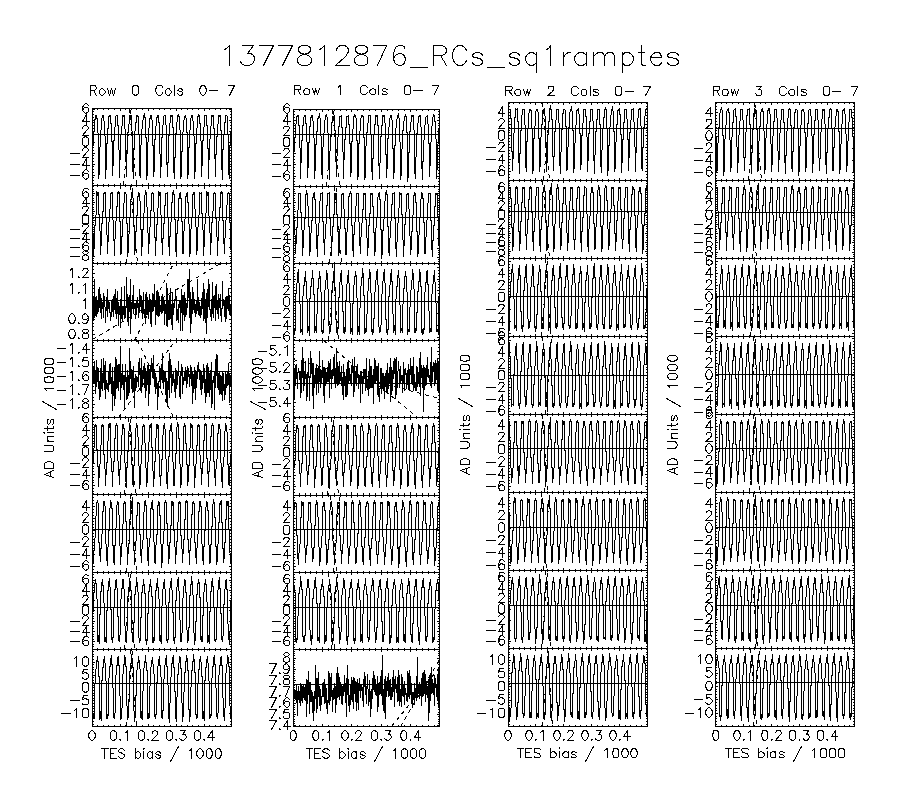
\includegraphics[width=\textwidth]{./images/1377812876_RCs_sq1ramptes_00.png}
\caption{Plot showing response of SQUID amplifier chain to ramp in \TES\ bias current, while \TES\ is superconducting. Data is shown for rows 0--4 for all eight columns. \RC{0}{2}, \RC{0}{3}, \RC{1}{3}, \RC{1}{7} all show no response, only noise (note the change in vertical scale for these row/columns). xxx need to explain units on axes?}
\label{fig:tes-bias-ramp-sc}
\end{figure*}

\begin{figure*}[th]
\centering
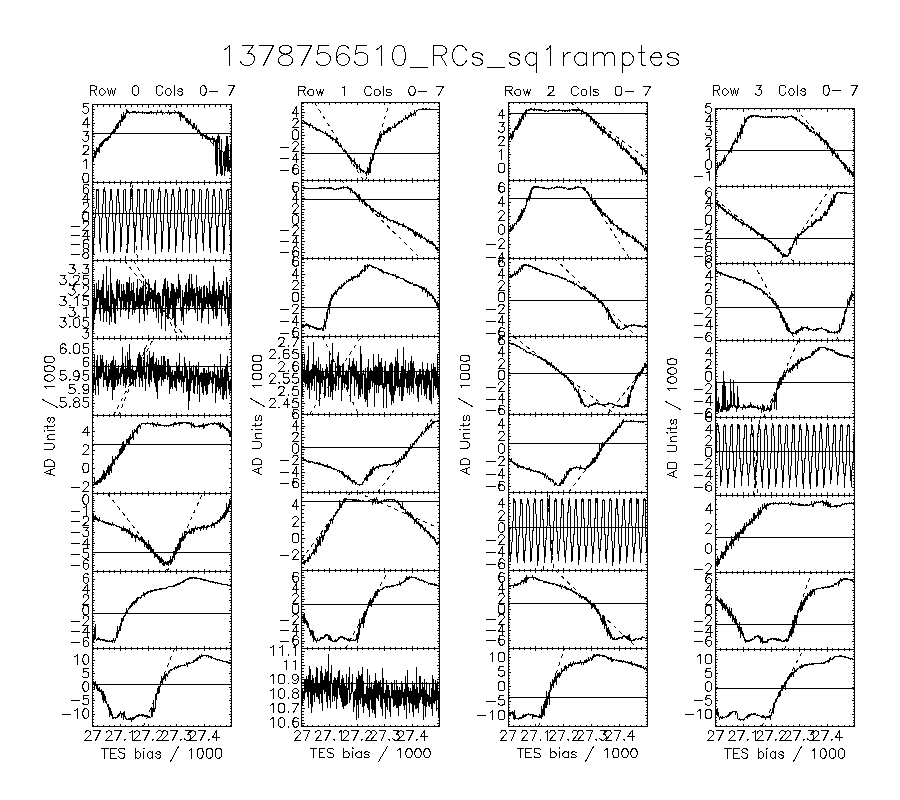
\includegraphics[width=\textwidth]{./images/1378756510_RCs_sq1ramptes_00.png}
\caption{Plot showing response of SQUID amplifier chain to ramp in \TES\ bias current, while \TES\ is biased into transition. The change in applied bias current is the same as in \figref{fig:tes-bias-ramp-sc}.
Data is shown for rows 0--4 for all eight columns.
\RC{0}{2}, \RC{0}{3}, \RC{1}{3}, \RC{1}{7} all show no response, only noise (note the change in vertical scale for these row/columns).
\RC{0}{1}, \RC{2}{5} and \RC{3}{4} all respond as if they were still superconducting (see \figref{fig:tes-bias-ramp-sc}).
The much slower mapping of the $V$-$\phi$ curve indicates a much higher resistance in the \TES\ circuit loop, due to the \TES\ itself starting to go normal.
xxx need to explain units on axes?}
\label{fig:tes-bias-ramp-trans}
\end{figure*}

\begin{figure*}
\centering
\includegraphics{./drawings/ch9-detector-cuts-wafer.pdf}
\caption{
Figure showing detector layout, highlighting which detectors have problems and which are working.
Each detector is labeled (below) with its row/column.
The x and y positions of the detectors on the wafer are also given, given in this thesis in the format X-Y, where X give the x position of the detector (labeled along the bottom) and Y the y position (labeled along the left).
}
\label{fig:detector-cuts-wafer}
\end{figure*}

\begin{figure*}
\centering
\includegraphics{./drawings/ch9-detector-cuts-rc.pdf}
\caption{Figure showing same information as \figref{fig:detector-cuts-wafer}, but organized in term of readout rows/columns. Each detector is labeled (below) with its position on the detector wafer. The rows/columns are labeled on the left and top. Unused row/columns as well as the row/columns used to readout the position of the secondary mirror are also indicated. }
\label{fig:detector-cuts-rc}
\end{figure*}


\section{Readout of Mirror Position}\label{s:mirror-readout}

The \Imager\ produces a time-ordered data stream containing the output of each detector as a function of time.
In order to turn this data stream into a video, we must know where the optical system is pointing at all times.
This pointing information is placed directly into the timestream by the \Imager, as described in this section.
It is also necessary to know where each detector is pointed relative to the optical system; this relative detector pointing information is extracted from beam maps, as discussed in \sectionref{s:beam-maps}.

The pointing of the optical system is set by the positions of the two actuators --- \DISP1 and \DISP2 --- that move the secondary mirror.
The actuator control hardware provides two voltage signal which are proportional to the positions of the actuators.
This voltage signal is sent into the \Imager\ cryostat by a pair coaxial cables.
Inside the cryostat two 1-m long Phosphur Bronze (xxx exact lakeshore name?) (PhBr) \AWG36 twisted pair wires carry the signal to the focal plane, where the signal is fed into the input coil of a 1st stage \SQUID.
Series resistors (\SI{4.23}{\mega\ohm} for \DISP1, \SI{4.36}{\mega\ohm} for \DISP2) are used at room temperature to reduce the current flowing through the wires to a value appropriate for the 1st stage \SQUID\ input; approximately \SI{10}{\uA}.

This approach allows the readout system to readout the position of the actuators in exactly the same way that it reads out the detector response.
The actuator position is synchronized perfectly with the detector data.

A natural question is whether cross-talk appears between the actuator readout and the other detectors.
To test this both actuator were moved in a 0.1~Hz sine-wave pattern over their maximum displacement range of +/- 3.5~mm, while the detectors were in the superconducting state.
Both actuators were moved at the same time, roughly \SI{135}{\degree} out of phase.
The level of crosstalk present can be quantified by performing a least-squares fit of each detector timestream $\vect{d}_{rc}$ to the model
\begin{equation}
	 \vect{d}_{rc} = A_1 \vect{d}_{\DISP1} + A_2 \vect{d}_{\DISP2}.
\end{equation}
Here $\vect{d}_{\DISP1}$ and $\vect{d}_{\DISP2}$ are the measured outputs for each actuator.
The maximum values of $|A_1|$  and $|A_2|$ are 0.0011 and 0.0014, respectively.
\figref{xxx} contains a plot summarizing these results.

An additional question is whether the actuator readout leads to higher noise.
xxx show results of this measurement.

% xxx - I get 500 uW for the load from these four wires (300 K - 1K). Can this be correct? I'm sure I did this calculation in the past and got a much smaller number. Did I screw up in the past? Is today's calculation in error? Am I intercepting this load at 50~K or 4~K, and I forgot about that? Did I use a much longer wire than 1~m? This could be a big cryogenic problem!

\section{Focus Distance}\label{s:focus-distance}

As described in \sectionref{s:optical-design}, the \Imager\ is designed to focus at distances of 16~m -- 30~m (xxx check 2nd distance).
All results described in this chapter were with the \Imager\ configured to focus at 16~m.
To check the actual distance to the target focal plane, beam maps as described in \sectionref{s:beam-maps} were performed with the blackbody source located at different distance from the cryostat.
\figref{fig:beam-vs-distance} shows beam maps for the same detector taken at different distances.
It is clear from this plot that the best focus occurs at \abt \SI{17}{m}, and the depth-of-field is approximately xxx~m.

The reasons for the difference from \ZEMAX\ predictions are not understood.
Possibilities include the cryostat being located too close to the primary mirror and the primary (or secondary) mirrors having an incorrect shape.

\section{Beam Maps}

As discussed in \sectionref{s:feedhorn-design}, the \Imager\ feedhorns are predicted to have beams that are circularly symmetric and well-approximated by Gaussians with \FWHM\ of x.xx~cm at the target.
To verify these predictions beam maps were performed by rastering the beams over a small, stationary \SI{1030}{\celsius} blackbody source.

The blackbody source used was an IR Labs xxx\footnote{IRLabs, Inc. Tucson, AZ. USA}.
This source reaches a maximum of \SI{1030}{\celsius} and has apertures ranging in size from x.xx in to x.xx in.
Best results were achieved by covering an area around the blackbody source with Aluminum foil; this eliminated hotspots in the image due to the warmth of the housing of the blackbody source itself.
\figref{xxx} shows a picture of the blackbody source with Aluminum foil mask.

The \Imager\ beams were rastered over the blackbody source by moving one actuator at xx~Hz while the other actuator moved much more slowly at xx~Hz.
This produces the path shown in \figref{xxx}.
The data stream for each detector was ``binned'' as described in \sectionref{xxx} to produce a beam map for each detector.
xxx did I remove any polynomials?
xxx need to discuss dimensional conversion factors
A 2-D Gaussian allowing for ellipticity was then fit to each beam map.
Only the points within xxx~cm of the map peak were included in the fit.

\figref{xxx} shows the resulting beam maps.
xxx describe this plot.

xxx compare to predictions.


\chapter{Vocab}

Placeholder for terms

\begin{description}
\item[``90~K'' Cold Plate]
\item[``4~K'' Cold Plate]
\item[Sorption Fridge]
\item[350~GHz Imager]
\item[PhBr]

\end{description}

\printbibliography

\end{document}
